\documentclass{llncs}

\usepackage{amsmath,amssymb,amsfonts}
\usepackage{graphicx}
\usepackage{xcolor, colortbl}
\usepackage{stmaryrd}
\usepackage{subcaption}
\usepackage{hyperref,cleveref}
\usepackage{tikz}

\usetikzlibrary{automata,positioning,shapes.multipart,arrows.meta}

\title{Flexible Runtime Security Enforcement with Tagged C}
\author{Sean Anderson \and Allison Naaktgeboren \and Andrew Tolmach}
\institute{Portland State University}

\begin{document}

\newcommand{\tagcolor}{C}

\newcommand{\vt}{\mathit{vt}}
\newcommand{\pt}{\mathit{pt}}
\newcommand{\lt}{\mathit{lt}}
\newcommand{\lts}{\overline{\lt}}
\newcommand{\nt}{\mathit{nt}}
\newcommand{\PCT}{\mathcal{P}}

\newcommand{\trule}[2]{#1 \leftarrow #2}

\newcommand{\truledef}[1]{
  & \multispan{3} \(#1\) \\}

\newcommand{\assert}[1]{& & & \multispan{2} \(\mathbf{assert} ~ #1\) \hfill \\}
\newcommand{\letin}[1]{& & & \multispan{2} \(\mathit{let} ~ #1 ~ \mathit{in}\) \\}

\newcommand{\caseof}[1]{\textnormal{case } #1 \textnormal{ of}}
\newcommand{\caseentry}[2]{& & & #1 \Rightarrow #2}

\newcommand{\optional}[1]{\fcolorbox{black}{gray!20}{#1}}
\newcommand{\settag}[2]{\boldsymbol{#1} & \longleftarrow & & \mathit{#2}\\}
\newcommand{\settagopt}[2]{\optional{\(\boldsymbol{#1}\)} & \longleftarrow & & \mathit{#2}\\}

%%% Tag Rules %%%
\newcommand{\loadtname}{\mathbf{LoadT}}
\newcommand{\loadtargs}{\PCT, \pt, \vt, \overline{\lt}}
\newcommand{\loadtres}{\vt'}
\newcommand{\loadt}{\loadtname(\loadtargs)}

\newcommand{\storetname}{\mathbf{StoreT}}
\newcommand{\storetargs}{\PCT, \pt, \vt_1, \vt_2, \overline{\lt}}
\newcommand{\storetres}{\PCT',\vt',\overline{\lt}'}
\newcommand{\storet}{\storetname(\storetargs)}

\newcommand{\consttname}{\mathbf{ConstT}}
\newcommand{\consttres}{\vt}
\newcommand{\constt}{\consttname}

\newcommand{\unoptname}{\mathbf{UnopT}}
\newcommand{\unoptargs}{\PCT, \vt}
\newcommand{\unoptres}{\vt}
\newcommand{\unopt}{\unoptname(\unoptargs)}

\newcommand{\binoptname}{\mathbf{BinopT}}
\newcommand{\binoptargs}{\PCT, \vt_1, \vt_2}
\newcommand{\binoptres}{\vt'}
\newcommand{\binopt}{\binoptname(\binoptargs)}

\newcommand{\globaltname}{\mathbf{GlobalT}}
\newcommand{\globaltargs}{id, s}
\newcommand{\globaltargstyped}{id \in ident, s \in \mathbb{N}}
\newcommand{\globaltres}{\pt,\vt,\overline{\lt}}
\newcommand{\globalt}{\globaltname(\globaltargs)}

\newcommand{\localtname}{\mathbf{LocalT}}
\newcommand{\localtargs}{\PCT, id, s}
\newcommand{\localtargstyped}{\PCT, id \in ident, s \in \mathbb{N}}
\newcommand{\localtres}{\pt,\vt,\overline{\lt}}
\newcommand{\localt}{\localtname(\localtargs)}

\newcommand{\vartname}{\mathbf{VarT}}
\newcommand{\vartargs}{\PCT, \vt}
\newcommand{\vartres}{\pt}
\newcommand{\vart}{\vartname(\vartargs)}

\newcommand{\malloctname}{\mathbf{MallocT}}
\newcommand{\malloctargs}{\PCT, \vt}
\newcommand{\malloctres}{\PCT',\pt,\optional{\(\vt,\overline{\lt}\)}}
\newcommand{\malloct}{\malloctname(\malloctargs)}

\newcommand{\freetname}{\mathbf{FreeT}}
\newcommand{\freetargs}{\PCT, \vt}
\newcommand{\freetres}{\PCT',\pt,\optional{\(\vt,\overline{\lt}\)}}
\newcommand{\freet}{\freetname(\freetargs)}

\newcommand{\picasttname}{\mathbf{PICastT}}
\newcommand{\picasttargs}{\PCT, \pt, \optional{\(\vt, \overline{\lt}\)}}
\newcommand{\picasttres}{\PCT',\vt}
\newcommand{\picastt}{\picasttname(\picasttargs)}

\newcommand{\ipcasttname}{\mathbf{IPCastT}}
\newcommand{\ipcasttargs}{\PCT, \vt_1, \optional{\(\vt_2, \overline{\lt}\)}}
\newcommand{\ipcasttres}{\PCT',\pt}
\newcommand{\ipcastt}{\ipcasttname(\ipcasttargs)}

\newcommand{\ppcasttname}{\mathbf{PPCastT}}
\newcommand{\ppcasttargs}{\PCT, \pt, \optional{\(\vt, \overline{\lt}\)}}
\newcommand{\ppcasttres}{\PCT',\pt'}
\newcommand{\ppcastt}{\picasttname(\picasttargs)}

\newcommand{\iicasttname}{\mathbf{IICastT}}
\newcommand{\iicasttargs}{\PCT, \vt_1}
\newcommand{\iicasttres}{\PCT',\pt}
\newcommand{\iicastt}{\ipcasttname(\ipcasttargs)}

\newcommand{\splittname}{\mathbf{SplitT}}
\newcommand{\splittargs}{\PCT, \vt, \optional{\(L\)}}
\newcommand{\splittres}{\PCT'}
\newcommand{\splitt}{\splittname(\splittargs)}
           
\newcommand{\jointname}{\mathbf{JointT}}
\newcommand{\jointargs}{\PCT, \optional{\(L\)}}
\newcommand{\jointres}{\PCT'}
\newcommand{\joint}{\jointname(\jointargs)}

\newcommand{\argtname}{\mathbf{ArgT}}
\newcommand{\argtargs}{\PCT, \vt, f, x}
\newcommand{\argtargstyped}{\PCT, \vt, f, x \in ident}
\newcommand{\argtres}{\vt'}
\newcommand{\argt}{\argtname(\argtargs)}

\newcommand{\callerrettname}{\mathbf{CallerRetT}}
\newcommand{\callerrettargs}{\PCT, \PCT', \vt}
\newcommand{\callerrettres}{\vt'}
\newcommand{\callerrett}{\callerrettname(\callerrettargs)}

\newcommand{\calleerettname}{\mathbf{CalleeRetT}}
\newcommand{\calleerettargs}{\PCT, \PCT', \vt}
\newcommand{\calleerettres}{\vt'}
\newcommand{\calleerett}{\calleerettname(\calleerettargs)}

%%%%%%%%%%%%%%%%%

%%% Continuations, States, Values %%%

\newcommand{\kemp}{\mathit{Kemp}}
\newcommand{\kdo}[1]{\mathit{Kdo};~ #1}
\newcommand{\kseq}[2]{\mathit{Kseq} ~ #1; ~ #2}
\newcommand{\kif}[4]{\mathit{Kif}[#1 \mid #2] ~ \mathit{join} ~ #3; ~ #4}
\newcommand{\kwhiletest}[4]{\mathit{KwhileTest}(#1) ~ \{ ~ #2 ~ \} ~ \mathit{join} ~ #3; ~ #4}
\newcommand{\kwhileloop}[4]{\mathit{KwhileLoop}(#1) ~ \{ ~ #2 ~ \} ~ \mathit{join} ~ #3; ~ #4}
\newcommand{\kdowhiletest}[4]{\mathit{KdoWhileTest}(#1) ~ \{ ~ #2 ~ \} ~ \mathit{join} ~ #3; ~ #4}
\newcommand{\kdowhileloop}[4]{\mathit{KdoWhileLoop}(#1) ~ \{ ~ #2 ~ \} ~ \mathit{join} ~ #3; ~ #4}
\newcommand{\kfor}[2]{\mathit{Kfor} ~ #1; ~ #2}
\newcommand{\kforpost}[2]{\mathit{KforPost} ~ #1; ~ #2}
\newcommand{\kcall}[3]{\mathit{Kcall} ~ #1 ~ #2 ~ #3}

\newcommand{\ctx}[1]{ctx \left[#1\right]}

\newcommand{\sstate}[6]{\mathcal{S}\left(f,#2,#3,#4 \mid #5 \gg #6 @ #1\right)}
\newcommand{\estate}[6]{\mathcal{E}\left(f,#2,#3,#4 \mid #5; \gg #6 @ #1\right)}
\newcommand{\cstate}[7]{\mathcal{C}\left(#1,#3,#4 \mid #5(#6) \gg #7 @ #2\right)}
\newcommand{\rstate}[6]{\mathcal{R}\left(#1,#3,#4 \mid #5 \gg #6 @ #2\right)}
\newcommand{\fstate}[1]{\mathcal{F}\left(#1\right)}

\newcommand{\mem}{m}
\newcommand{\genv}{\mathit{ge}}
\newcommand{\lenv}{\mathit{le}}
\newcommand{\cont}{k}
\newcommand{\stmt}{s}
\newcommand{\expr}{e}
\newcommand{\type}{ty}
\newcommand{\defestate}[1]
           {\estate{\PCT}{\mem}{\genv}{\lenv}{#1}{\cont}}
\newcommand{\defsstate}[1]
           {\sstate{\PCT}{\mem}{\genv}{\lenv}{#1}{\cont}}

\newcommand{\valof}[1]{|#1|}
\newcommand{\deref}[1]{* #1}
\newcommand{\addrof}[1]{\& #1}
\newcommand{\assignop}[3]{#2 ~~ [#1]\!\!= #3}
\newcommand{\postinc}[2]{#2 #1\!\!#1}
\newcommand{\assign}[2]{#1 := #2}
\newcommand{\loc}[2]{\underline{#1}@#2}
\newcommand{\val}[2]{\mathit{#1} @ #2}
\newcommand{\binop}[3]{#2 #1 #3}
\newcommand{\unop}[2]{#1 #2}
\newcommand{\comma}[2]{#1, #2}
\newcommand{\paren}[2]{(#2) (#1)}
\newcommand{\builtin}[2]{\mathit{builtin} ~ #1(#2)}
\newcommand{\var}[1]{#1}
\newcommand{\cast}[2]{(#2) #1}
\newcommand{\call}[2]{#1(#2)}
\newcommand{\condition}[3]{#1 ~ ? ~ #2 ~ : ~ #3}
\newcommand{\sizeof}[1]{\mathtt{size}(#1)}
\newcommand{\alignof}[1]{\mathtt{align}(#1)}

\newcommand{\sskip}{\mathtt{skip}}
\newcommand{\sdo}[1]{#1;}
\newcommand{\sseq}[2]{#1 ~ #2}
\newcommand{\scontinue}{\mathtt{continue}}
\newcommand{\sbreak}{\mathtt{break}}
\newcommand{\sreturn}{\mathtt{return}}
\newcommand{\sifthenelse}[4]{\mathtt{if}(#1) ~ \mathtt{then} ~ #2 ~ \mathtt{else} ~ #3 ~ \mathtt{join} ~ #4}
\newcommand{\swhile}[3]{\mathtt{while}(#1) ~ \mathtt{do} ~ #2 ~ \mathtt{join} ~ #3}
\newcommand{\sdowhile}[3]{\mathtt{do} ~ #2 ~ \mathtt{while} ~ (#1) ~ \mathtt{join} ~ #3}
\newcommand{\sfor}[5]{\mathtt{for}(#1; #2; #3) ~ \mathtt{do} ~ #4 ~ \mathtt{join} ~ #5}
\newcommand{\sswitch}[2]{\mathtt{switch} ~ #1 ~ \{ ~ #2 ~ \}}
\newcommand{\slabel}[2]{#1: ~ #2}
\newcommand{\sgoto}[1]{\mathtt{goto} ~ #1}

\newcommand{\vundef}{\mathbf{undef}}

\newcommand{\tptr}[1]{\mathit{ptr(#1)}}

\newcommand{\judgment}[3][]{
  {\centering
  \smallskip
  \begin{tabular}{c}
    #2 \\
    \hline
    #3
  \end{tabular}{\sc #1}
  \smallskip\par}}

\newcommand{\judgmentbr}[4][]{
  {\centering
  \smallskip
  \begin{tabular}{c}
    #2 \\
    #3 \\
    \hline
    #4
  \end{tabular}{\sc #1}
   \smallskip\par}}

\newcommand{\judgmentbrbr}[5][]{
  {\centering
  \smallskip
  \begin{tabular}{c}
    #2 \\
    #3 \\
    #4 \\
    \hline
    #5
  \end{tabular}{\sc #1}
   \smallskip\par}}

\newcommand{\judgmentbrbrbr}[6][]{
  {\centering
  \smallskip
  \begin{tabular}{c}
    #2 \\
    #3 \\
    #4 \\
    #5 \\
    \hline
    #6
  \end{tabular}{\sc #1}
   \smallskip\par}}

\newcommand{\judgmenttwobr}[6][]{
  {
    \centering
    \smallskip
    \begin{tabular}{c c}
       #2 & #3 \\
       #4 & #5 \\
       \hline
       \multicolumn{2}{c}{#6}
    \end{tabular}{\sc #1}
    \vspace{\belowdisplayskip}\par
  }}

\newcommand{\judgmenttwobrlong}[5][]{
  {
    \centering
    \smallskip
    \begin{tabular}{c c}
       #2 & #3 \\
       \multicolumn{2}{c}{#4} \\
       \hline
       \multicolumn{2}{c}{#5}
    \end{tabular}{\sc #1}
    \vspace{\belowdisplayskip}\par
  }}

\newcommand{\judgmentthreebrlong}[6][]{
  {
    \centering
    \smallskip
    \begin{tabular}{c c c}
       #2 & #3 & #4 \\
       \multicolumn{3}{c}{#5} \\
       \hline
       \multicolumn{3}{c}{#6}
    \end{tabular}{\sc #1}
    \vspace{\belowdisplayskip}\par
  }}

\newcommand{\judgmentthreebrtwo}[7][]{
  {
    \centering
    \smallskip
    \begin{tabular}{c c c}
       #2 & #3 & #4 \\
       \multicolumn{3}{c}{#5 \hfill #6} \\
       \hline
       \multicolumn{3}{c}{#7}
    \end{tabular}{\sc #1}
    \vspace{\belowdisplayskip}\par
  }}

\newcommand{\judgmenttwobrlongbrlong}[6][]{
  {
    \centering
    \smallskip
    \begin{tabular}{c c}
       #2 & #3 \\
       \multicolumn{2}{c}{#4} \\
       \multicolumn{2}{c}{#5} \\
       \hline
       \multicolumn{2}{c}{#6} \\
    \end{tabular}{\sc #1}
    \vspace{\belowdisplayskip}\par
  }}


\newcommand{\judgmentthreebr}[8][]{
  {
    \centering
    \smallskip
    \begin{tabular}{c c c}
       #2 & #3 & #4 \\
       #5 & #6 & #7 \\
       \hline
       \multicolumn{3}{c}{#8}
    \end{tabular}{\sc #1}
    \vspace{\belowdisplayskip}\par
  }}


\newcommand{\judgmenttwo}[4][]{
  {\centering
  \smallskip
  \begin{tabular}{c c}
    #2 & #3 \\
    \hline
    \multicolumn{2}{c}{#4}
  \end{tabular}{\sc #1}
  \smallskip\par}}

\newcommand{\judgmentthree}[5][]{
  {\centering
  \smallskip
  \begin{tabular}{c c c}
    #2 & #3 & #4 \\
    \hline
    \multicolumn{3}{c}{#5}
  \end{tabular}{\sc #1}
  \smallskip\par}}

\newcommand{\judgmentfour}[6][]{
  {\centering
  \smallskip
  \begin{tabular}{c c c c}
    #2 & #3 & #4 & #5 \\
    \hline
    \multicolumn{4}{c}{#6}
  \end{tabular}{\sc #1}
  \smallskip\par}}

\newcommand{\truleblock}[2]
           {
             \tcbox{
             \begin{tabular}{l}
               #1 \\
               #2 \\
             \end{tabular}}
           }

\newcommand{\malloctname}{\color{blue} \mathbf{MallocT}}
\newcommand{\malloctargs}{\PCT, \pt, \vt}
\newcommand{\malloctres}{\PCT['],\pt['],\vt['],\lt[']}
\newcommand{\malloct}{\malloctname(\malloctargs)}

\newcommand{\malloctruleblock}[1]
           {
             \truleblock{\(\malloct\)}{#1}
           }

\newcommand{\localtname}{\color{blue} \mathbf{LocalT}}
\newcommand{\localtargs}{\PCT, \TN}
\newcommand{\localtres}{\PCT['], \pt['], \lt[']}
\newcommand{\localt}{\localtname(\localtargs)}

\newcommand{\localtruleblock}[1]
           {
             \truleblock{\(\localt\)}{#1}
           }

\newcommand{\accesstname}{\color{blue} \mathbf{AccessT}}
\newcommand{\accesstargs}{\PCT,\vt}
\newcommand{\accesstres}{\vt[']}
\newcommand{\accesst}{\accesstname(\accesstargs)}

\newcommand{\accesstruleblock}[1]
           {
             \truleblock{\(\accesst\)}{#1}
           }

\newcommand{\loadtname}{\color{blue} \mathbf{LoadT}}
\newcommand{\loadtargs}{\PCT, \pt, \vt, \lt}
\newcommand{\loadtres}{\vt[']}
\newcommand{\loadt}{\loadtname(\loadtargs)}

\newcommand{\loadtruleblock}[1]
           {
             \truleblock{\(\loadt\)}{#1}
           }

\newcommand{\assigntname}{\color{blue} \mathbf{AssignT}}
\newcommand{\assigntargs}{\PCT,\vt[_1],\vt[_2]}
\newcommand{\assigntres}{\PCT['],\vt[']}
\newcommand{\assignt}{\assigntname(\assigntargs)}

\newcommand{\assigntruleblock}[1]
           {
             \truleblock{\(\assignt\)}{#1}
           }
           
\newcommand{\storetname}{\color{blue} \mathbf{StoreT}}
\newcommand{\storetargs}{\PCT, \pt, \vt, \lt}
\newcommand{\storetres}{\PCT['],\vt['],\lt[']}
\newcommand{\storet}{\storetname(\storetargs)}

\newcommand{\storetruleblock}[1]
           {
             \truleblock{\(\storet\)}{#1}
           }

\newcommand{\unoptname}{\color{blue} \mathbf{UnopT}}
\newcommand{\unoptargs}{\odot, \PCT, \vt}
\newcommand{\unoptres}{\vt[']}
\newcommand{\unopt}{\unoptname(\unoptargs)}
           
\newcommand{\unoptruleblock}[2]
           {
             \colorbox{blue!10}{
               \begin{tabular}{l}
                 \(\unopt\) \\
                 % body
                 #1 \\
                 % outputs
                 \{ \(\unoptres\) \} \\
               \end{tabular}
             }
           }
           
\newcommand{\binoptname}{\color{blue} \mathbf{BinopT}}
\newcommand{\binoptargs}{\oplus, \PCT, \vt[_1], \vt[_2]}
\newcommand{\binoptexargs}{\oplus,\vt[_1],\vt[_2]}
\newcommand{\binoptres}{\vt[']}
\newcommand{\binopt}{\binoptname(\binoptargs)}
\newcommand{\binoptex}{\binoptname(\binoptexargs)}

\newcommand{\binoptruleblock}[1]
           {
             \truleblock{\(\binopt\)}{#1}
           }

\newcommand{\binoptexruleblock}[1]
           {
             \truleblock{\(\binoptex\)}{#1}
           }

           
\newcommand{\calltname}{\color{blue} \mathbf{CallT}}
\newcommand{\calltargs}{\PCT, \pt}
\newcommand{\calltres}{\PCT[']}
\newcommand{\callt}{\calltname(\calltargs)}
           
\newcommand{\calltruleblock}[1]
           {
             \truleblock{\(\callt\)}{#1}
           }

\newcommand{\argtname}{\color{blue} \mathbf{ArgT}}
\newcommand{\argtargs}{\PCT, \vt, \FN, \AN}
\newcommand{\argtexargs}{\vt,\FN,\AN}
\newcommand{\argtres}{\PCT['], \vt[']}
\newcommand{\argt}{\argtname(\argtargs)}
\newcommand{\argtex}{\argtname(\argtexargs)}

\newcommand{\argtruleblock}[1]
           {
             \truleblock{\(\argt\)}{#1}
           }

\newcommand{\argtexruleblock}[1]
           {
             \truleblock{\(\argtex\)}{#1}
           }
           
\newcommand{\rettname}{\color{blue} \mathbf{RetT}}
\newcommand{\rettargs}{\PCT[_{\color{blue} CLE}], \PCT[_{\color{blue} CLR}], \vt}
\newcommand{\rettres}{\PCT['],\vt[']}
\newcommand{\rett}{\rettname(\rettargs)}

\newcommand{\rettruleblock}[1]
           {
             \truleblock{\(\rett\)}{#1}
           }

\newcommand{\consttname}{\color{blue} \mathbf{ConstT}}
\newcommand{\consttargs}{\PCT}
\newcommand{\consttres}{\vt[']}
\newcommand{\constt}{\consttname(\consttargs)}

\newcommand{\consttruleblock}[1]
           {
             \truleblock{\(\constt\)}{#1}
           }

\newcommand{\inittname}{{\color{blue} \mathbf{InitT}}}
\newcommand{\inittargs}{\PCT}
\newcommand{\inittres}{\vt[']}
\newcommand{\initt}{\inittname(\inittargs)}

\newcommand{\inittruleblock}[1]
           {
             \truleblock{\(\initt\)}{#1}
           }
           
\newcommand{\globaltname}{\color{blue} \mathbf{GlobalT}}
\newcommand{\globaltargs}{\GN, \TN}
\newcommand{\globaltres}{\pt['],\vt['],\lt[']}
\newcommand{\globalt}{\globaltname(\globaltargs)}

\newcommand{\globaltruleblock}[1]
           {
             \truleblock{\(\globalt\)}{#1}
           }

\newcommand{\dealloctname}{\color{blue} \mathbf{DeallocT}}
\newcommand{\dealloctargs}{\PCT, \TN}
\newcommand{\dealloctres}{\PCT['],\vt['],\lt[']}
\newcommand{\dealloct}{\dealloctname(\dealloctargs)}

\newcommand{\freetname}{\color{blue} \mathbf{FreeT}}
\newcommand{\freetargs}{\PCT,\pt,\vt}
\newcommand{\freetres}{\PCT['],\vt['],\lt[']}
\newcommand{\freet}{\freetname(\freetargs)}

\newcommand{\picasttname}{\color{blue} \mathbf{PICastT}}
\newcommand{\picasttargs}{\PCT, \pt, \lt, \TN}
\newcommand{\picasttres}{\vt[']}
\newcommand{\picastt}{\picasttname(\picasttargs)}

\newcommand{\picasttruleblock}[1]
           {
             \truleblock{\(\picastt\)}{#1}
           }

\newcommand{\ipcasttname}{\color{blue} \mathbf{IPCastT}}
\newcommand{\ipcasttargs}{\PCT, \vt, \lt, \TN}
\newcommand{\ipcasttres}{\pt[']}
\newcommand{\ipcastt}{\ipcasttname(\ipcasttargs)}

\newcommand{\ipcasttruleblock}[1]
           {
             \truleblock{\(\ipcastt\)}{#1}
           }

\newcommand{\ppcasttname}{\color{blue} \mathbf{PPCastT}}
\newcommand{\ppcasttargs}{\PCT, \pt[_1], \pt[_2], \lt[_1], \lt[_2], \TN}
\newcommand{\ppcasttres}{\pt[']}
\newcommand{\ppcastt}{\ppcasttname(\ppcasttargs)}

\newcommand{\iicasttname}{\color{blue} \mathbf{IICastT}}
\newcommand{\iicasttargs}{\PCT, \vt[_1], \TN}
\newcommand{\iicasttres}{\pt[']}
\newcommand{\iicastt}{\iicasttname(\iicasttargs)}

\newcommand{\splittname}{\color{blue} \mathbf{SplitT}}
\newcommand{\splittargs}{\PCT, \vt, \LN}
\newcommand{\splittres}{\PCT[']}
\newcommand{\splitt}{\splittname(\splittargs)}

\newcommand{\splittruleblock}[1]
           {
             \truleblock{\(\splitt\)}{#1}
           }

\newcommand{\exprsplittname}{\color{blue} \mathbf{ExprSplitT}}
\newcommand{\exprsplittargs}{\PCT, \vt}
\newcommand{\exprsplittres}{\PCT[']}
\newcommand{\exprsplitt}{\exprsplittname(\exprsplittargs)}

\newcommand{\exprsplittruleblock}[1]
           {
             \colorbox{blue!10}{
               \begin{tabular}{l}
                 \(\exprsplitt\) \\
                 #1 \\
               \end{tabular}
             }
           }


\newcommand{\exprjointname}{\color{blue} \mathbf{ExprJoinT}}
\newcommand{\exprjointargs}{\PCT, \vt}
\newcommand{\exprjointres}{\PCT['], \vt[']}
\newcommand{\exprjoint}{\exprjointname(\exprjointargs)}

\newcommand{\exprjointruleblock}[1]
           {
             \colorbox{blue!10}{
               \begin{tabular}{l}
                 \(\exprjoint\) \\
                 #1 \\
               \end{tabular}
             }
           }

\newcommand{\labeltname}{\color{blue} \mathbf{LabelT}}
\newcommand{\labeltargs}{\PCT, \LN}
\newcommand{\labeltres}{\PCT[']}
\newcommand{\labelt}{\labeltname(\labeltargs)}

\newcommand{\labeltruleblock}[1]
           {
             \truleblock{\(\labelt\)}{#1}
           }

\newcommand{\extcalltname}{\color{blue} \mathbf{ExtCallT}}
\newcommand{\extcalltargs}{\PCT, \pt, \overline{\vt}}
\newcommand{\extcalltres}{\PCT[']}
\newcommand{\extcallt}{\extcalltname(\extcalltargs)}

\newcommand{\fieldtname}{\color{blue} \mathbf{FieldT}}
\newcommand{\fieldtargs}{\PCT, \pt, \TN, \GN}
\newcommand{\fieldtres}{\pt[']}
\newcommand{\fieldt}{\fieldtname(\fieldtargs)}

%%%%%%%%%%%%%%%%%

\newcommand{\caseofthree}[7]
           {
             \begin{tabular}{l c l}
               \multicolumn{3}{l}{\textnormal{case } #1 \textnormal{ of}} \\
               #2 & \(\Rightarrow\) & #3 \\
               #4 & \(\Rightarrow\) & #5 \\
               #6 & \(\Rightarrow\) & #7 \\
             \end{tabular}
           }

\newcommand{\caseoftwo}[5]
           {
             \begin{tabular}{l c l}
               \multicolumn{3}{l}{\textnormal{case } #1 \textnormal{ of}} \\
               #2 & \(\Rightarrow\) & #3 \\
               #4 & \(\Rightarrow\) & #5 \\
             \end{tabular}
           }

\newcommand{\mallocstep}
{\judgmenttwobrlong
    {\(\trule{\malloctres}{\malloct}\)}
    {\(\mem',p \leftarrow \mathit{heap\_alloc} ~ \mathit{size} ~ \mem\)}
    {\(\mem'' = \mem'\left[p + i \mapsto (\vundef,\vt,\lt) \mid 0 \leq i < s\right]\)}
    {\(\defestate{\ctx{\mathit{malloc(\mathit{size}@t)}}}
      \longrightarrow
      \estate{\PCT'}{\mem''}
             {\ctx{\val{p}{\pt}}}{\cont}\)}}

\newcommand{\valofstep}
{\judgmenttwo{\(\mem[l]_{|ty|} = v@\vt@\overline{\lt}\)}
            {\(\trule{\loadtres}{\loadt}\)}
            {\(\estate{\PCT}{\mem}
              {\ctx{\valof{\loc{l}{\pt}}}}{\cont}
              \longrightarrow
              \estate{\PCT}{\mem}
                     {\ctx{\val{v}{\vt'}}}{\cont}\)}}

\newcommand{\assignopstep}
{\judgmenttwobr{\(\mem[l]_{|ty|} = v_1@\vt @\overline{\lt}\)}
  {\(\oplus \in \{+,-,*,/,\%,<<,>>,\&,^\wedge,|\}\)}
  {\(\trule{\loadtres}{\loadt}\)}
  {\(\expr = \assign{\loc{l}{\pt}}
    {\binop{\oplus}
      {\val{v_1}{\vt'}}
      {\val{v_2}{\vt_2}}}\)}
  {\(\defestate
    {\ctx{\assignop{\oplus}{\loc{l}{\pt}}
        {\val{v_2}{\vt_2}}}}
    \longrightarrow
    \defestate
        {\ctx{\expr}}\)}}

\newcommand{\postincstep}
{\judgmentthreebrtwo{\(\mem[l] = v@\vt @\overline{\lt}\)}
               {\(\oplus \in \{+,-\}\)}
               {\(\trule{\loadtres}{\loadt}\)}
               {\(\trule{\consttres}{\constt}\)}
               {\(\expr = \comma{\assign{\loc{l}{\pt}}{\binop{\oplus}{\val{v}{\vt'}}{1@\constt}}}
                 {\val{v}{\vt'}} \)}
               {\(\defestate
                 {\ctx{\postinc{\oplus}
                     {\loc{l}{\pt}}}}
                 \longrightarrow
                 \defestate
                     {\ctx{\expr}}\)}}

\newcommand{\assignstep}
{\judgmenttwobrlong{\(\mem[l]_{|ty|} = v_1@\vt_1@\overline{\lt}\)}
                  {\(\mem' = \mem[l \mapsto v_2@\vt' @\overline{\lt}']\)}
                  {\(\trule{\storetres}{\storet}\)}
                  {\(\defestate
                    {\ctx{\assign{\loc{l}{\pt}}{\val{v_2}{\vt_2}}}}
                    \longrightarrow
                    \estate{\PCT'}{\mem'}
                           {\ctx{\val{v_2}{\vt_2}}}{\cont}\)}}

\newcommand{\varstep}
{\judgmenttwo{\(\lenv[id] = (l,\_,\pt,ty)\)}
  {\(\trule{\vartres}{\vart}\)}
  {\(\defestate{\ctx{\var{id}}}
    \longrightarrow
    \defestate{\ctx{\loc{l}{\pt}}}\)}}

\newcommand{\unopstep}
{\judgmenttwo{\(\left\langle \odot \right\rangle v = v'\)}
            {\(\vt' = \unopt{\PCT}{\vt}\)}
            {\(\defestate{\ctx{\unop{\odot}{\val{v}{\vt}}}}
              \longrightarrow
              \defestate{\ctx{\val{v'}{\vt'}}}\)}}

\newcommand{\binopstep}
{\judgmenttwo{\(v_1 \left\langle \oplus \right\rangle v_2 = v'\)}
            {\(\vt' = \binopt{\PCT}{\vt_1}{\vt_2}\)}
            {\(\defestate{\ctx{\binop{\oplus}{\val{v_1}{\vt_1}}{\val{v_2}{\vt_2}}}}
              \longrightarrow
              \defestate{\ctx{\val{v'}{\vt'}}}\)}}

\newcommand{\dostepa}
{\judgment{}
  {\(\defsstate{\expr;} \longrightarrow
    \estate{\PCT}{\mem}{\expr}{\kdo{\cont}}\)}
}

\newcommand{\dostepb}
{\judgment{}
  {\(\estate{\PCT}{\mem}{\val{v}{\vt}}{\kdo{\cont}} \longrightarrow
    \defsstate{\sskip}\)}
}

\newcommand{\seqstep}
{\judgment{}
  {\(\defsstate{\stmt_1;\stmt_2} \longrightarrow
    \sstate{\PCT}{\mem}{\stmt_1;}{\kseq{\stmt_2}{\cont}}\)}
}

\newcommand{\seqskipstep}
{\judgment{}
  {\(\sstate{\PCT}{\mem}{\sskip}{\kseq{\stmt}{\cont}} \longrightarrow
    \defsstate{\stmt}\)}
}

\newcommand{\seqcontinuestep}
{\judgment{}
  {\(\sstate{\PCT}{\mem}{\scontinue}{\kseq{\stmt}{\cont}} \longrightarrow
    \sstate{\PCT}{\mem}{\scontinue}{\cont}\)}}

\newcommand{\seqbreakstep}
{\judgment{}
  {\(\sstate{\PCT}{\mem}{\sbreak}{\kseq{\stmt}{\cont}} \longrightarrow
    \sstate{\PCT}{\mem}{\sbreak}{\cont}\)}}

\newcommand{\ifstepa}
{\judgment{\(\stmt=\sifthenelse{\expr}{\stmt_1}{\stmt_2}{L}\)}
  {\(\defsstate{\stmt} \longrightarrow
    \estate{\PCT}{\mem}{\expr}{\kif{\stmt_1}{\stmt_2}{L}{\cont}}\)}
}

\newcommand{\ifstepb}
{\judgmenttwo
  {\(\stmt' =
    \begin{cases}
      \stmt_1 & \textnormal{if } \mathit{boolof}(v) = \mathbf{t} \\
      \stmt_2 & \textnormal{if } \mathit{boolof}(v) = \mathbf{f} \\
    \end{cases}\)}
  {\(\trule{\splittres}{\splitt}\)}
  {\(\estate{\PCT}{\mem}{\val{v}{\vt}}{\kif{\stmt_1}{\stmt_2}{L}{\cont}}
    \longrightarrow
    \sstate{\PCT'}{\mem}{\stmt'}{\cont}\)}
}

\newcommand{\whilestep}
{\judgment{\(\stmt=\swhile{\expr}{\stmt'}{L}\)}
  {\(\defsstate{\stmt} \longrightarrow
    \estate{\PCT}{\mem}{\expr}{\kwhiletest{\expr}{\stmt'}{L}{\cont}}\)}
}

\newcommand{\whiletruestep}
{\judgmentthree
  {\(\mathit{boolof}(v) = \mathbf{t}\)}
  {\(\cont_1 = \kwhiletest{\expr}{\stmt}{L}{\cont}\)}
  {\(\cont_2 = \kwhileloop{\expr}{\stmt}{L}{\cont}\)}
  {\(\estate{\PCT}{\mem}{\val{v}{\vt}}{\cont_1}
    \longrightarrow
    \sstate{\PCT'}{\mem}{\stmt}{\cont_2}\)}
}

\newcommand{\whilefalsestep}
{\judgmenttwo
  {\(\mathit{boolof}(v) = \mathbf{f}\)}
  {\(\cont = \kwhiletest{\expr}{\stmt}{L}{\cont'}\)}
  {\(\estate{\PCT}{\mem}{\val{v}{\vt}}{\cont}
    \longrightarrow
    \sstate{\PCT'}{\mem}{\sskip}{\cont'}\)}
}

\newcommand{\whileskipcontinuestep}
{\judgmenttwo{\(\stmt = \sskip \lor \stmt = \scontinue\)}
  {\(\cont = \kwhileloop{\expr}{\stmt}{L}{\cont'}\)}
  {\(\defsstate{\stmt} \longrightarrow
    \sstate{\PCT}{\mem}{\swhile{\expr}{\stmt}{L}}{\cont'}\)}}

\newcommand{\whilebreakstep}
{\judgment{\(\cont = \kwhileloop{\expr}{\stmt}{L}{\cont'}\)}
  {\(\sstate{\PCT}{\mem}{\sbreak}{\cont} \longrightarrow
    \sstate{\PCT}{\mem}{\sskip}{\cont'}\)}}

\newcommand{\dowhilestep}
{\judgmenttwo{\(\stmt = \sdowhile{\expr}{\stmt}{L}\)}
  {\(\cont' = \kdowhileloop{\expr}{\stmt}{L}{\cont}\)}
  {\(\defsstate{\stmt} \longrightarrow
    \sstate{\PCT}{\mem}{\stmt}{\cont'}\)}
}

\newcommand{\dowhileskipcontinuestep}
{\judgmenttwo
  {\(\cont_1 = \kdowhileloop{\expr}{\stmt}{L}{\cont'}\)}
  {\(\cont_2 = \kdowhiletest{\expr}{\stmt}{L}{\cont}\)}
  {\(\sstate{\PCT}{\mem}{\stmt' = \sskip \lor \stmt' = \scontinue}{\cont_1} \longrightarrow
    \estate{\PCT}{\mem}{\expr}{\cont_2}\)}}

\newcommand{\dowhiletruestep}
{\judgmenttwo
  {\(\mathit{boolof}(v) = \mathbf{t}\)}
  {\(\cont = \kdowhiletest{\expr}{\stmt}{L}{\cont'}\)}
  {\(\estate{\PCT}{\mem}{\val{v}{\vt}}{\cont}
    \longrightarrow
    \sstate{\PCT'}{\mem}{\sdowhile{\expr}{\stmt}{L}}{\cont'}\)}
}

\newcommand{\dowhilefalsestep}
{\judgmenttwo
  {\(\mathit{boolof}(v) = \mathbf{f}\)}
  {\(\cont = \kdowhiletest{\expr}{\stmt}{L}{\cont'}\)}
  {\(\estate{\PCT}{\mem}{\val{v}{\vt}}{\cont}
    \longrightarrow
    \sstate{\PCT'}{\mem}{\sskip}{\cont'}\)}
}

\newcommand{\dowhilebreakstep}
{\judgment{\(\cont = \kdowhileloop{\expr}{\stmt}{L}{\cont'}\)}
  {\(\sstate{\PCT}{\mem}{\sbreak}{\cont} \longrightarrow
    \sstate{\PCT}{\mem}{\sskip}{\cont'}\)}}

\newcommand{\forinitstep}
{\judgmenttwo
  {\(\stmt = \sfor{\stmt_1}{\expr}{\stmt_2}{\stmt_3}{L}\)}
  {\(\stmt_1 \not = \sskip\)}
  {\(\defsstate{\stmt} \longrightarrow
  \sstate{\PCT}{\mem}{\stmt_1}{\kseq{\sfor{\sskip}{\expr}{\stmt_2}{\stmt_3}{L}}{\cont}}\)}
}

\newcommand{\forstep}
{\judgment{\(\stmt = \sfor{\sskip}{\expr}{\stmt_2}{\stmt_3}{L}\)}
  {\(\defsstate{\stmt} \longrightarrow
  \estate{\PCT}{\mem}{\expr}{\kfor{\stmt}{\cont}}\)}
}

\newcommand{\forfalsestep}
{\judgment{\(\mathit{boolof}(v) = \mathbf{f}\)}
  {\(\estate{\PCT}{\mem}{\val{v}{\vt}}{\kfor{\stmt}{\cont}} \longrightarrow
    \sstate{\PCT}{\mem}{\sskip}{\cont}\)}
}

\newcommand{\fortruestep}
{\judgmenttwo{\(\stmt = \sfor{\sskip}{\expr}{\stmt_2}{\stmt_3}{L}\)}
             {\(\mathit{boolof}(v) = \mathbf{t}\)}
  {\(\estate{\PCT}{\mem}{\val{v}{\vt}}{\kfor{\stmt}{\cont}} \longrightarrow
      \sstate{\PCT}{\mem}{\stmt_3}{\kfor{\stmt}{\cont}}\)}
}

\newcommand{\forskiporcontinuestep}
{\judgmenttwo{\(\stmt = \sfor{\sskip}{\expr}{\stmt_1}{\stmt_2}{L}\)}
  {\(\stmt = \sskip \lor \stmt = \scontinue\)}
  {\(\sstate{\PCT}{\mem}{\stmt}{\kfor{\stmt}{\cont}}
    \longrightarrow
    \sstate{\PCT}{\mem}{\stmt_1}{\kforpost{\sfor{\sskip}{\expr}{\stmt_1}{\stmt_2}{L}}{\cont}}\)}
}

\newcommand{\forbreakstep}
{\judgment{\(\stmt = \sfor{\sskip}{\expr}{\stmt_1}{\stmt_2}{L}\)}
  {\(\sstate{\PCT}{\mem}{\sbreak}{\kfor{\stmt}{\cont}}
    \longrightarrow
    \sstate{\PCT}{\mem}{\sskip}{\cont}\)}
}
  
\newcommand{\forskippoststep}
{\judgment{\(\stmt = \sfor{\sskip}{\expr}{\stmt_1}{\stmt_2}{L}\)}
  {\(\sstate{\PCT}{\mem}{\sskip}{\kforpost{\stmt}{\cont}}
    \longrightarrow
    \defsstate{\stmt}\)}
}

\newcommand{\callexprstep}
{\judgment{}
  {\(\estate{\PCT}{\mem}{\ctx{\call{f'}{\overline{v @ \vt}}}}{ty}{\cont}
    \longrightarrow
    \cstate{f'}{\PCT}{\mem}{\genv}{\lenv}{v @ \vt}{\kcall{f}{\ctx}{\cont}}\)}
}

\newcommand{\retvalstep}
{\judgment{\(\mathit{pop} ~ \cont = \kcall{f'}{\ctx}{\cont'}\)}
  {\(\sstate{\PCT}{\mem}{\sreturn ~ \val{v}{\vt}}{\cont}
    \longrightarrow
    \rstate{f'}{\PCT}{\mem}{\genv}{\val{v}{\vt}}{\ctx}{\cont}\)}
}

\newcommand{\callstep}
{\judgmentbr{\(\mathit{def}(f) = (xs, \stmt)\)}
  {\(\lenv' = \lenv \llbracket x \mapsto v@\vt' \mid
    (x,v@\vt) \leftarrow \mathit{zip}(xs,args), \vt' \leftarrow \argt \rrbracket\)}
  {\(\cstate{f}{\PCT}{\mem}{\genv}{\lenv}{args}{\cont} \longrightarrow
    \sstate{\PCT}{\mem}{\genv}{\lenv'}{\stmt}{\cont}\)}}

\newcommand{\returnstep}
{\judgmenttwo{\(\cont = \mathit{Kcall} ~ \lenv' ~ \mathit{ctx} ~ \cont'\)}
  {\(\PCT'',\vt' \leftarrow \rett\)}
  {\(\rstate{\PCT}{\mem}{\genv}{\lenv}{\val{v}{\vt}}{\cont} \longrightarrow
    \estate{\PCT'}{\mem}{\mathit{ctx}[\val{v}{\vt'}]}{\cont'}\)}}

\newcommand{\labelstep}
{\judgment
  {\(\jointres \leftarrow \joint \)}
  {\(\sstate{\PCT}{\mem}
    {L: \stmt}{\cont} \longrightarrow
    \sstate{\PCT'}{\mem}{\genv}{\lenv'}{\stmt}{\cont}\)}}

\newcommand{\memory}[4]
           {             
             \begin{tabular}{|c|c|c|c|}
               \multicolumn{4}{l}{#1} \\
               \hline
               \multicolumn{4}{|c|}{#2 \(@\) #3} \\
               \hline
               \footnotesize #4 & \footnotesize #4 & \footnotesize #4 & \footnotesize #4 \\
               \hline
             \end{tabular}
           }
           
\newcommand{\memoryA}
           {
             node {\memory{1000}{\(\vundef\)}{\(\N\)}{\(\N\)}}; \&
             node {\memory{1004}{\(\vundef\)}{\(\N\)}{\(\N\)}}; \&
             node {\memory{1008}{\(\vundef\)}{\(\N\)}{\(\N\)}}; \&
             node {\memory{1092}{\(\vundef\)}{\(\N\)}{\(\N\)}}; \&
             node {\memory{1096}{\(\vundef\)}{\(\N\)}{\(\N\)}}; \\
           }


\maketitle

\begin{abstract}
Today's computing infrastructure is built atop layers of legacy C code, often
insecure, poorly understood, and/or difficult to maintain.
These foundations may be shored up with dynamic security enforcement,
which spares legacy code owners from having to modify their code.
% and potentially introduce regressions.
Tagged C is a C variant with a built-in {\em tag-based reference monitor} for use in expressing
a variety of dynamic security policies and enforcing them with compiler and hardware support.

Tagged C is comprehensive in the policies that it can support. In this paper we will discuss
{\em memory safety}, {\em compartmentalization}, and {\em secure information flow} (SIF)
policies. It is flexible in covering the tradeoff between conservative policies that may
halt too many programs and more permissive ones. And as a source language, it should be
more accessible to C programmers than existing assembly-level tag-based reference monitors.

\end{abstract}

\section{Introduction}
Many essential technologies rely on new and old C code. 
Operating systems (Linux, Windows, OSX, BSD), databases (Oracle, sqlite3), the internet \&
web (Apache, NGNIX, NetBSD, Cisco IOS), the Internet of Things (IoT), and the 
embedded devices that run our homes and hospitals are built in and on C \cite{Munoz:PoweredbyC}. 
C is not a relic; more than a third of professional programmers report active developing
in C today \cite{stackoverflow22:dev-survey}. The safety of public and private systems we depend on every day
in turn depends on the security of their underlying C codebases. Insecurity might take the form
of undefined behavior such as memory errors, of logic errors such as sql injection or other
input-sanitization flaws, or of larger-scale architectural flaws that over-provision components of the
system with privilege.

Although static analyses can detect and mitigate many C insecurities, the last line of defense against
undetected or unfixable vulnerabilities is dynamic enforcement at runtime. Ideally an engineer can
tune enforcement to the security needs of the system, rather than apply one-size-fits-all conservative
restrictions. To allows developers to define flexible security policies in terms of a familiar source language,
we introduce Tagged C: a general-purpose dynamic tag-based enforcement language.
Applications of Tagged C include giving precise definition to undefined behaviors (UBs) involving memory,
specifying detailed information flow policies, and enforcing arbitrary mandatory access control tables.
Importantly, a security policy can be modified without recompilation unless it is optimized as described in
\cref{sec:optionals}.

The novelty of Tagged C is that it is a \emph{general-purpose} scheme for specifying security
policies at the source level, using a tag-based reference monitor.
This style of monitor associates a metadata tag with the data in the underlying system,
and throughout execution it updates these tags according to a set a predefined rules, or halts if
the program would violate a rule. This is the underlying concept of PIPE, an ISA extension that
implements a reference monitor in hardware, as well as similar systems such as ARM MTE and
[that thing from Binghamton]. While our scheme is general and could be implemented in software,
we are motivated by PIPE and aim for compatibility with it as a likely hardware target.

Tagged C consists of an underlying semantics that establishes the baseline concrete behavior of programs
with no policies, and a set of {\em control points} at which the semantics consult a user defined set of
{\em tag rules}. For convenience we build our underlying semantics on the CompCert C semantics, which are formalized 
as part of the CompCert verified compiler \cite{Leroy09:CompCert}. We provide a reference interpreter
also based on that of CompCert, for use executing prototype policies.

\paragraph{Contributions}

We offer the following contributions:

\begin{itemize}
\item A full formal semantic definition for Tagged C, formalized in Coq
\item The design of a comprehensive set of {\em control points} at which the language interfaces with the policy
\item A Tagged C interpreter, implemented in Coq and extracted to Ocaml
\item Tagged C policies implementing (1) compartmentalization,
  (2) a realistic, permissive memory model from the literature (PVI),
  and (3) Secure Information Flow (SIF)
\end{itemize}

In the next section, we give a high-level introduction of metadata-tagging: how it works,
and how its use can improve security. Then in \cref{sec:semantics}, we briefly discuss the
language as a whole, before moving into policies in \cref{sec:policies}. Finally, in
\cref{sec:evaluations} we discuss the degree to
which the design meets our goals of flexibility and applicability to realistic
security concerns.

\section{What is Metadata Tagging?}
  
Consider a very simple security requirement: ``do not leak the password.''
For simplicity, we will suppose that {\tt pwd} is an integer in this case, and consider
a number of ways that it might be leaked (\cref{fig:exampleleak}).
In example (a), we store it in a local variable, then pass it to {\tt printf}.
In (b), we perform some arithmetic on it before printing it, but an observer could
easily determine the original value. In (c), we store it to a volatile variable
representing an mmapped region. And in (d), we loop over it, and store the loop
counter in the same mmapped variable, indirectly revealing the value.

To prevent example (a), we need to keep track of the value of the input as it
moves from its initial temporary variable to the stack and then is passed, and
we need to check the origins of any value we pass to {\tt printf}. Example (b)
further requires that we track the provenance of the value as we perform arithmetic
on it.

Example (c) reveals that we need to separately track some information about memory
locations in addition to the values that they hold, and example (d) asks us to track
how the overall state has been influenced by {\tt pwd}.

% Other options: (1) cursor pointing at lines of code
% (2) table of te/mem states, corresponding to lines of code
% Introduce rules by name from the beginning
% Call out how we attach P to pwd (introduce name tags)
% Text explaining diagrams
% Elide byte-level description, explain that we're cheating later

\begin{figure}
  \begin{subfigure}[t]{0.49\textwidth}
\begin{verbatim}
void f(int pwd) {
  int x = pwd;
  printf("%d", x);
}
\end{verbatim}
\caption{}
\label{fig:ex1}
  \end{subfigure}  
  \begin{subfigure}[t]{0.49\textwidth}
\begin{verbatim}
volatile int mm;

void g(int pwd) {
  if (pwd > 128) {
    mm = i;
  }
}
\end{verbatim}
\caption{}
\label{fig:ex2}
  \end{subfigure}

  \caption{Examples of leaking {\tt pwd}}
  \label{fig:exampleleak}
\end{figure}

Lets examine the program state at various points as we execute example \ref{fig:ex1}.
Let the value of \(\mathit{pwd}\) be represented by the variable \(i\). We consider this
value to be high-security, and wish to track it as it moves through the system, distinguishing
it from other, low-security values. These security levels, which we will write \high 
and \low, form our set of {\em tags} that represent important metadata about
a value in the program. On entry to {\tt f}, we assign tags to both the parameter {\tt pwd}
and the local variable {\tt x}, based on the \(\argtname\) and \(\localtname\) tag rules,
respectively. We will call these \(\vt_1\) and \(\vt_2\), as they are tags on values.
\(\localtname\) takes as its parameter the identity of the function being entered, and \(\argtname\)
takes the tag \(\vt_0\) on the value being passed into {\tt f} as well as the identities of both the
function and the argument. Next, we load \(i\) from {\tt pwd} and store it in {\tt x}, and we need to
consult tag rules, \(\loadtname\) and \(\storetname\). Finally, when we make the call to
{\tt printi}, we once again consult \(\argtname\).

\begin{tikzpicture}[every text node part/.style={align=left}]
  \node[matrix, ampersand replacement=\&, anchor=west] (code)
       {
         \node (l1) {\tt void f(int pwd) \{}; \\
         \node (l2) {\tt ~ ~ int x = pwd+5;}; \\
         \node (l3) {\tt ~ ~ printi(x);}; \\
         \node {\tt \}}; \\
       };
       
  \node[matrix, ampersand replacement=\&, node distance=6em, right=of l1.north,draw,anchor=west] (table1)
       {
         \node[anchor=north] {\(f\)}; \&
         \node[anchor=north] {\(\mathtt{x} \mapsto \vundef @ \vt_1\) \\ \(\mathtt{pwd} \mapsto i @ \vt_2\)}; \&
         \node[anchor=north] {\(\vt_1 \leftarrow \localtname(f)\) \\ \(\vt_2 \leftarrow \argtname(\vt_0,f,pwd)\)};\\
       };

  \node[matrix, ampersand replacement=\&, node distance=4.5em, below=of table1.west,draw,anchor=west] (table2)
       {
         \node[anchor=north] {\(f\)}; \&
         \node[anchor=north] {\(\mathtt{x} \mapsto (i+5) @ \vt_5\) \\ \(\mathtt{pwd} \mapsto i @ \vt_2\)}; \&
         \node[anchor=north] {\(\vt_3 \leftarrow \loadtname(\vt_2)\) \\
           \(\vt_4 \leftarrow \binoptname(+,\vt_3,\constt)\) \\
           \(\vt_5 \leftarrow \storetname(\vt_4)\)}; \\
       };

  \node[matrix, ampersand replacement=\&, node distance=4.5em, below=of table2.west,draw,anchor=west] (table3)  
       {
         \node[anchor=north] {\(\mathit{printi}\)}; \&
         \node[anchor=north] {\(\mathtt{a} \mapsto i @ \vt_7\)}; \&
         \node[anchor=north] {\(\vt_6 \leftarrow \loadtname(\vt_5)\) \\
           \(\vt_7 \leftarrow \argtname(\vt_6, \mathit{printi}, a)\)}; \\
       };

  \draw[Circle-]
  (l1.south) -| (table1.west);

  \draw[Circle-]
  (l2.south) -| (table2.west);

  \draw[Circle-]
  (l3.south) |- (table3.west);  

\end{tikzpicture}

These points at which the tags are checked and either propagated or updated by tag rules are termed
{\em control points}. Collectively, the tag rules form a {\em policy}. Now we define a
``don't print {\tt pwd}'' policy that tracks the influence of {\tt pwd} and failstops if it would
leak. The tag set, as previously noted, consists of the high and low tags, and we define our critical
tag rules as follows.

\begin{minipage}{0.3\textwidth}
  \begin{align*}
  \tau::=\high | \low \\
  \constt = \low \\
  \localtname(f) = \low \\
  \loadtname(\vt) = \vt \\
  \storetname(\vt) = \vt \\
  \end{align*}
\end{minipage}
\begin{minipage}{0.6\textwidth}
\begin{align*}
  \binoptname(\oplus,\vt_1,\vt_2) = \begin{cases} \low & \textnormal{if } \vt_1 = \vt_2 = \low \\
    \high & \textnormal{otherwise} \end{cases}\\
  \argtname(\vt, f, id) = \begin{cases} \fail & \textnormal{if } f=\mathtt{printi} \textnormal{ and } \vt = \high \\
    \high & \textnormal{if } f=\mathtt{f} \textnormal{ and } id = \mathtt{pwd} \\
    \vt & \textnormal{otherwise} \\
  \end{cases} \\
\end{align*}
\end{minipage}

As we see, most of the tagrules simply move tags around. The most interesting ones are \(\binoptname\),
which combines two tags, setting the result of a binary operation \(\high\) if either of its arguments are,
and \(\argt\). \(\argt\) checks whether the function being called is {\tt printi} and fails if it is
and the value being passed is tagged \high. It also always tagged {\tt pwd} \high, and otherwise it just maintains
the security level of the input it is given. So, in this example, we will be unable to generate a tag
\(\vt_7\), and the tag processor will throw a failstop rather than allow execution to continue.

Example \ref{fig:ex2} adds two new wrinkles: we need to keep track of metadata associated with
addresses and with the program's control-flow state. If the volatile variable {\tt mm} represents
mmapped memory that can be seen publicly, we want to avoid storing the password there. And, by
branching on the password, we risk leaking information that could eventually compromise it even
if we never print it directly (an {\em implicit flow}.) So we extend our state with additional
``location tags'' on memory locations, which we will range over with \(\lt\) by convention.
Meanwhile, pointers, including those that are the static addresses of local or global variables,
will be given tags ranged over by \(\pt\). Finally, to track metadata associated with the program's
control flow, we maintain a special global tag called the PC Tag, ranged over by \(\PCT\).

\begin{tikzpicture}[every text node part/.style={align=left}]
  \node[matrix, ampersand replacement=\&, anchor=west] (code)
       {
         \node {\tt volatile int mm;}; \\
         \node (l1) {\tt void g(int pwd) \{}; \\
         \node (l2) {\tt ~ ~ if(pwd > 0)}; \\
         \node (l3) {\tt ~ ~ ~ ~ mm = 1;}; \\
         \node {\tt \}}; \\
       };

  \node[matrix, ampersand replacement=\&, node distance=6em, right=of l1.north,draw,anchor=west] (table1)  
       {
         \node[anchor=north] {\(g @ \PCT_1\)}; \&
         \node[anchor=north] {\(\mathtt{mm} @ \pt_1 \mapsto \vundef @ \vt_1 @ \lt_1\) \\
         \(\mathtt{pwd} @ \pt_2 \mapsto i @ \vt_2\)}; \&
         \node[anchor=north] {\(\pt_1, \vt_1,\lt_1 \leftarrow \globaltname(mm)\) \\
           \(\pt_2, \vt_2 \leftarrow \argtname(\vt_0,g,pwd)\) \\
           \(\PCT_1 \leftarrow \calltname(\PCT_0, g)\)}; \\
       };
       
 \node[matrix, ampersand replacement=\&, node distance=5em, below=of table1.west,draw,anchor=west] (table2)         
      {
        \node[anchor=north] {\(g @ \PCT_2\)}; \&
        \node[anchor=north] {\(\mathtt{mm} @ \pt_1 \mapsto \vundef @ \vt_1 @ \lt_1\) \\
          \(\mathtt{pwd} @ \pt_2 \mapsto i @ \vt_2 @ \lt_2\)}; \&
        \node[anchor=north] {\(\vt_3 \leftarrow \constt\) \\
          \(\vt_4 \leftarrow \binoptname(>,\vt_2,\vt_3)\) \\ 
          \(\PCT_2 \leftarrow \splittname(\PCT_1, \vt_4)\)}; \\
      };

 \node[matrix, ampersand replacement=\&, node distance=4.5em, below=of table2.west,draw,anchor=west] (table3)         
      {
        \node[anchor=north] {\(g @ \PCT_2\)}; \&
        \node[anchor=north] {\(\mathtt{mm} @ \pt_1 \mapsto 1 @ \vt_5 @ \lt_3\) \\
          \(\mathtt{pwd} @ \pt_2 \mapsto i @ \vt_2 @ \lt_2\)}; \&
        \node[anchor=north] {\(\vt_4 \leftarrow \constt\) \\
          \(\vt_5,\lt_3 \leftarrow \storetname(\PCT_2,\pt_1,\vt_1,\vt_4,\lt_1)\)}; \\
      };

  \draw[Circle-]
  (l1.south) -| (table1.west);

  \draw[Circle-]
  (l2.south) -| (table2.west);

  \draw[Circle-]
  (l3.south) |- (table3.west);  

\end{tikzpicture}

Here, we initialize the tags on {\tt mm} with the \(\globaltname\) rule. The PC Tag
at the point of call, \(\PCT_0\), is fed to the \(\calltname\) rule to determine a new PC Tag
inside of {\tt g}. And the if-statement consults the \(\splittname\) rule to update the PC Tag
inside of its branch based on the value-tag of the expression {\tt pwd < 0}. Once inside the
loop, we perform the store, taking into account all of the additional tags.

To upgrade our ``don't print the password'' policy to ``don't leak the password,'' we can
keep most of our rules the same, or extend them in natural ways. Crucially, we will tag memory
locations \high by default, indicating that they are allowed to contain \high-tagged values,
but {\tt mm} will be tagged \low. The most interesting rules are:

\begin{align*}
  \globaltname(id) =
  \begin{cases}
    \low, \low, \low & \textnormal{if } id = \mathtt{mm} \\
    \low, \low, \high & \textnormal{otherwise} \\
  \end{cases} &
  \splittname(\PCT,\vt) =
  \begin{cases}
    \low & \textnormal{if } \vt = \PCT = \low \\
    \high & \textnormal{otherwise} \\
  \end{cases} \\
\end{align*}
\[\storet = \begin{cases}
  \fail & \textnormal{if } \PCT = \high \textnormal { or } \vt_2 = \high \textnormal{ and } \lt = \low \\
  \low, \high & \textnormal{if } \PCT = \vt_2 = \low \\
  \high, \high & \textnormal{otherwise} \\
\end{cases}\]
\[\argtname(\vt, f, id) = \begin{cases} \fail & \textnormal{if } f=\mathtt{printi} \textnormal{ and } \vt = \high \\
  \high, \high & \textnormal{if } f=\mathtt{g} \textnormal{ and } id = \mathtt{pwd} \\
  \vt, \high & \textnormal{otherwise} \\
\end{cases}\]

In this case, \(\splittname\) will set the PC Tag to \high, as it branches on a value derived from {\tt pwd}.
Then, when it comes time to write to {\tt mm}, \(\storetname\) will fail rather than write to a low address
in a high context.

\section{The Language, Informally}

Tagged C uses the full syntax of CompCert C \cite{Leroy09:CompCert} with minimal modification (\cref{fig:syntax}).
There are two notable syntactical differences in the language, relative to CompCert C:
conditionals and loops take an optional {\em join point} label, and parenthetical expressions
an optional ``context tag.''

Our semantics are a small-step reduction semantics which differ from CompCert C's in
two key respects. These are given in full in the appendix. First, Tagged C's semantics contain
{\em control points}: hooks within the
operational semantics at which the tag policy is consulted and either tags are updated, or the system
failstops. (Control points resemble ``advice points'' in aspect-oriented programming, but narrowly
focused on the manipulation of tags.) A control point consists of the name of a {\em tag rule}
and the bindings of its inputs and outputs; a tag rule is a partial function. The names and
signatures of the tag rules, and their corresponding control points, are listed in \Cref{fig:controlpoints}.

Second, there is no memory-undefined behavior: the source semantics reflect a
concrete target-level view of memory as a flat address space. Without memory safety, programs
that exhibit memory-undefined behavior will act as their compiled equivalents would, potentially
corrupting memory; we expect that a memory safety policy will be a standard default, but that the
strictness of the policy may need to be tuned for programs that use low-level idioms.

The choice of control points and their associations with tag rules, as well as the tag rules'
signatures, are a crucial design element. Our proposed design is sufficient for the three classes of
policy that we explore in this paper, but it may not be complete.

\section{Tags and Policies}
\label{sec:policies}

Tagged C can enforce a wide range of policies, as follows.
A policy consists of a tag type \(\tau\), a default tag inhabiting that type, and an instantiation
of each tag rule identified in \cref{fig:controlpoints}. Tags in gray boxes are optional, as discussed
in \cref{sec:optionals}.

\begin{table}[t]
  \begin{tabular}{|l|l|l|l|}
    \hline
    Rule Name & Inputs & Outputs & Control Points \\
    \hline
    \(\loadtname\)      & \(\loadtargs\)         & \(\loadtres\)      & Memory Loads \\
    \(\storetname\)     & \(\storetargs\)        & \(\storetres\)     & Memory Stores \\
    \(\unoptname\)      & \(\unoptargs\)         & \(\unoptres\)      & Unary Operation \\
    \(\binoptname\)     & \(\binoptargs\)        & \(\binoptres\)     & Binary Operation \\
    \(\consttname\)     &                        & \(\consttres\)     & Applied to Constants/Literals \\
    \(\exprsplittname\) & \(\exprsplittargs\)    & \(\exprsplittres\) & Control-flow split points in expressions \\
    \(\exprjointname\)  & \(\exprjointargs\)     & \(\exprjointres\)  & Join points in expressions \\
    \(\splittname\)     & \(\splittargs\)        & \(\splittres\)     & Control-flow split points in statements)\\
    \(\labeltname\)     & \(\labeltargs\)        & \(\labeltres\)     & Labels/arbitrary code points \\
    \(\calltname\)      & \(\calltargs\)         & \(\calltres\)      & Call \\
    \(\argtname\)       & \(\argtargs\)          & \(\argtres\)       & Call \\
    \(\rettname\)       & \(\rettargs\)          & \(\rettres\)       & Return \\
    \(\globaltname\)    & \(\globaltargs\)       & \(\globaltres\)    & Program initialization \\
    \(\localtname\)     & \(\localtargs\)        & \(\localtres\)     & Call \\
    \(\dealloctname\)   & \(\dealloctargs\)      & \(\dealloctres\)   & Return \\
    \(\extcalltname\)   & \(\extcalltargs\)      & \(\extcalltres\)   & Call to linked code \\
    \(\malloctname\)    & \(\malloctargs\)       & \(\malloctres\)    & Call to {\tt malloc} \\
    \(\freetname\)      & \(\freetargs\)         & \(\freetres\)      & Call to {\tt free} \\
    \(\fieldtname\)     & \(\fieldtargs\)        & \(\fieldtres\)     & Field Access \\
    \(\picasttname\)    & \(\picasttargs\)       & \(\picasttres\)    & Cast from pointer to scalar \\
    \(\ipcasttname\)    & \(\ipcasttargs\)       & \(\ipcasttres\)    & Cast from scalar to pointer \\
    \(\ppcasttname\)    & \(\ppcasttargs\)       & \(\ppcasttres\)    & Cast between pointers \\
    \(\iicasttname\)    & \(\iicasttargs\)       & \(\iicasttres\)    & Cast between scalars \\
    \hline
  \end{tabular}

  \caption{Full list of tag-rules in control points}
  \label{fig:controlpoints}
\end{table}

\paragraph*{Name Tags}

When we want to define a per-program policy, we need to be able to attach tags to the program's
functions, globals, and so on. We do this by automatically embedding their identifiers in tags,
which are available to all policies. These are called {\em name tags}. We give name tags to the
following constructions and identify them as follows:
\begin{itemize}
\item Function identifiers, \(\FN\)
\item Function arguments, \(\AN\)
\item Global variables, \(\GN\)
\item Labels, \(\LN\)
\item Types, \(\TN\)
\end{itemize}

\subsection{PVI Memory Safety}
\label{sec:PVI}

Our first policy is a form of memory safety that uses the ``provenance via integer'' (PVI) memory model
of Memarian et al. \cite{Memarian19:ExploringCSemantics}.
Variations of memory safety have been enforced in PIPE already, but usually using
an ad hoc memory model. PVI has the virtue of giving definition to many memory UBs in which a pointer is
cast to an integer, subjected to various arithmetic operations, and cast back to a pointer.
Their second memory model, {\it PNVI} (provenance not via integer), is even more permissive.
We can also enforce it in Tagged C, though its security value is questionable, and we will
not describe it in this paper.

When we say that we want to enforce this specific memory model, we mean that our policy should
not failstop on any program that is defined in PVI, and that it should failstop if and when a program
reaches undefined behavior. So, in the following examples, we would like {\tt mark} to proceed without
failing, while {\tt overflow} should failstop.

\begin{minipage}{0.65\textwidth}
\begin{verbatim}
int mark(uintptr ptr) {
  if (!(ptr & 0x00000001))
    *(int*) (ptr | 0x11111110) = 0;

  return ((uintptr) ptr | 0x00000001);
}
\end{verbatim}
\end{minipage}
\begin{minipage}{0.34\textwidth}
\begin{verbatim}
void overflow() {
  int[3] x;
  int y;
  *x = 222222;
  *(x+10) = 333333;
}
\end{verbatim}
\end{minipage}

Both code snippets are undefined behavior in C, but {\tt mark} is a common low-level
idiom \cite{Memarian16:DeFacto}, seen for example in implementations of Cheney's garbage collection algorithm.
Taking advantage of the fact that objects in memory are four-aligned, it
uses the lower-order bits of the pointer to store a flag. In this case, it first checks
the flag, and if it is not set, it zeroes the memory and then sets it. This is generally
considered to be harmless, in contrast to {\tt overflow}, where {\tt y} is being overwritten
due to being adjacent in memory to {\tt x}. Here we show the state of the local environment
(mapping identifiers to addresses and pointer tags) and memory:

\begin{tikzpicture}[every text node part/.style={align=left}]
  \node[matrix, ampersand replacement=\&, anchor=west] (code)
       {
         \node (l0) {\tt void overflow() \{}; \\
         \node (l1) {\tt ~ ~ int[3] x; int y;}; \\
         \node (l2) {\tt ~ ~ *x = 222222;}; \\
         \node (l3) {\tt ~ ~ *(x+3) = 333333;}; \\
         \node {\tt \}}; \\
       };

  \node[matrix, ampersand replacement=\&, node distance=4em, right=of l1.east,draw,anchor=west] (table1)
       {
         \node[anchor=north]{\(\mathit{overflow} @ \PCT_2\)}; \&
         \node[anchor=north]{\(\mathtt{x}\mapsto \underline{84} @ \pt_1)\) \\ \(\mathtt{y} \mapsto \underline{96} @ \pt_2\)}; %\&
         %         \node[anchor=north] {\(\vt_1 \leftarrow \localtname(f)\) \\ \(\vt_2 \leftarrow \argtname(\vt_0,f,pwd)\)};
         \\
       };

  \node[matrix, ampersand replacement=\&, column sep=-1em, node distance=4em, below=of l3.west,anchor=west] (table2)
       {
         \node[anchor=north] {\hspace{1em}}; \&
         \node[anchor=north] {\memory{\(84\)}{\(\vundef\)}{\(\vt_1\)}{\(\lt_1\)}}; \&
         \node[anchor=north] {\memory{\(88\)}{\(\vundef\)}{\(\vt_1\)}{\(\lt_1\)}}; \&
         \node[anchor=north] {\memory{\(92\)}{\(\vundef\)}{\(\vt_1\)}{\(\lt_1\)}}; \&
         \node[anchor=north] {\memory{\(96\)}{\(\vundef\)}{\(\vt_2\)}{\(\lt_2\)}};
         \\
       };

  \node[matrix, ampersand replacement=\&, column sep=-1em, node distance=4em, below=of table2.west,anchor=west] (table3)
       {
         \node[anchor=north] {\hspace{1em}}; \&
         \node[anchor=north] {\memory{\(84\)}{\(222222\)}{\(\vt_3\)}{\(\lt_3\)}}; \&
         \node[anchor=north] {\memory{\(88\)}{\(\vundef\)}{\(\vt_1\)}{\(\lt_1\)}}; \&
         \node[anchor=north] {\memory{\(92\)}{\(\vundef\)}{\(\vt_1\)}{\(\lt_1\)}}; \&
         \node[anchor=north] {\memory{\(96\)}{\(333333\)}{\(\vt_4\)}{\(\lt_4\)}};
         \\
       };

       
\end{tikzpicture}

We now show separate location tags on each of the four bytes in each word. In the inputs and outputs
of a tag rule, we write this \(\lts\), indicating that the rule consumes and produces multiple locations tags.
If the PC Tag is \(\PCT_0\) when we enter the function,
our initial tags come from \(\PCT_1,\pt_1,\vt_1,\lts_1 \leftarrow \localtname(\PCT_0,\TN[int])\)
followed by \(\PCT_2,\pt_2,\vt_2,\lts_2 \leftarrow \localtname(\PCT_1,\TN[int])\).

The write to {\tt *(x+3)} is of particular interest. We tag the result of {\tt x+3}
with \(\pt' \leftarrow \binoptname(\PCT_2, \pt_1, \constt)\); then for the store itself,
we use the rule \(\vt_4, \lts_4 \leftarrow \storetname(\PCT_2, \pt', \vt_2, \constt, \lts_2)\).

We can prevent overflows like this using a {\em memory safety} policy. In brief, whenever
an object is allocated, it is assigned a unique ``color,'' and its memory locations as well
as its pointer are tagged with that color. Pointers maintain their tags under arithmetic
operations, and loads and stores are legal if the pointer matches the target memory location.
The rules for the \(PVI\) memory safety policy are given in \cref{fig:pvi}. In this case, we will
have \(\pt_1 = \lt_1 = \tagz\) and \(\pt_2 = \lt_2 = \tagone\). When we try to write to {\tt x+3},
we compare \(\pt' = \tagz\) with \(\lt_2\), and failstop because they differ.

\begin{figure}
  \color{blue}
  \begin{align*}
    \tau ::= & \clr & \clr \in \mathbb{N} \\
    & \N \\
  \end{align*}
  
  \scriptsize
  \begin{minipage}[t]{0.3\textwidth}
    \vspace{-2.5em}
    \binoptruleblock{
      \caseofthree
          {\((\vt_1,~ \vt_2)\)}
          {\((\gentag,\N)\)}{\(\vt' := \gentag\)}
          {\((\N,\gentag)\)}{\(\vt' := \gentag\)}
          {\((\clr_1, \clr_2)\)}{\(\vt' := \N\)}
    }
    \unoptruleblock{\(\vt' := \vt\)}

  \end{minipage}
  \begin{minipage}[t]{0.25\textwidth}
    \vspace{-2.5em}
    \localtruleblock
        {\(\PCT' := \PCT+1\);
          \(\pt := \PCT\)\\
          \(\vt := \N\);
          \(\lts := \left[ \PCT \right]\)
        }
    \malloctruleblock
        {\(\PCT' := \PCT+1\);
          \(\pt := \PCT\) \\
          \(\vt := \N\);
          \(\lts := \left[ \PCT \right]\)
        }
  \end{minipage}
  \begin{minipage}[t]{0.3\textwidth}
    \vspace{-2.5em}
    \loadtruleblock{\(\mathbf{assert} ~ \forall \lt \in \overline{\lt} . \pt = \lt\) \\ \(\vt' := \vt\)}

    \storetruleblock{\(\mathbf{assert} ~ \forall \lt \in \lts . \pt = \lt\) \\
      \(\PCT' := \PCT\);
      \(\vt' := \vt_2\); 
      \(\lts' := \lts\)}
  \end{minipage}

  \caption{PVI Memory Safety Policy}
  \label{fig:pvi}
\end{figure}

The cast rules, meanwhile, have no effect on the tag of the value being cast at all. So,
we can cast a pointer to a scalar value, perform any operation that is defined on that type
on it, and cast it back, and it will retain its pointer tag. As long as it ends up pointing
at the same object, loads and stores will be successful. Function pointers are an exception:
Tagged C's underlying control-flow protections prevent them from being tampered with.

\subsection{Compartmentalization}
\label{sec:comp}
% notes ended up below, in the coarse grained section
In a perfect world, all C programs would be memory safe. But it is unfortunately common
for a codebase to contain undefined behavior that will not be fixed, including memory undefined
behavior. This may occur because developers intentionally use low-level idioms that are UB
\cite{Memarian16:DeFacto}, or because the cost and risk of regressions may make it
undesirable to fix bugs in older code,
as opposed to code under active development that is held to a higher standard \cite{Bessey10:Coverity}.

A compartmentalization policy isolates potentially risky code, such as code with known UB,
from safety-critical code, minimizing the damage that can be done if a vulnerability is exploited.
It may also contain restricts on how code in one part of the system may interact with another
even in the absence of language-level errors---ideally, restricting each component to the
{\em least privilege} necessary to complete its task.
This common form of protection can be implemented at many levels. It is often built
into a system's fundamental design, like a web browser sandbox untrusted javascript.
But for our use-case, we consider a compartmentalization scheme being added to the system
after the fact.

Let's assume that we have a set of compartment identifiers, ranged over by \(C\), and a mapping
from function identifiers to compartments, \(\mathit{comp}(f)\). This mapping must be provided by
a security engineer.

\paragraph{Coarse-grained Protection}

% this is two tasks in the same process, all they want to do is pass scalars adn not stomp
% on each other
% then fine grained is libaries + your code, which usually need more
% than mere scalars. think libc. could foil rop gadgets? 
% mac - explicit list of allowed calls
% capability - says this is shared, protects with basic safety. anything 
%   else cannot be shared. unique colors to defeat forced pointer arthimetic. hybrid system
%   roughly the effect of containing things, but wihtout the issues of the MAC
%
The core of a compartmentalization scheme is once again memory protection. For the simplest version,
we will enforce that memory allocated by a function is only accessible by functions that share its
compartment. To do that, we need to keep track of which compartment we're in, using the PC Tag.

Calls and returns each take two steps: first to an intermediate call or return state, and
then to the normal execution state, as shown in \cref{fig:functions} with some function \(f\)
calling \(f'\). In the initial call step, \(\calltname\)
uses the name-tags of the caller and callee to update the PC Tag. Then, in the step from the call
state, we place the function arguments in the temp environment, tagging their values with
the results of \(\argtname\), and we allocate our stack locals, tagging their values and locations
with the results of \(\localtname\). And on return, we deallocate locals and update their location
tags with \(\dealloctname\) when stepping to a return state, and from there \(\rettname\) updates both
the PC Tag and the tag on the returned value.

\begin{figure}
  \begin{tikzpicture}[]
    \node[state]                                      (f)                           {$f$};
    \node[state, inner sep = 0pt, minimum size = 0pt] (call) [above right=of f]     {$\mathcal{C}$};
    \node[state]                                      (g)    [below right=of call]  {$f'$};
    \node[state, inner sep = 0pt, minimum size = 0pt] (ret)  [below right=of f]     {$\mathcal{R}$};
    
    \path[->]
    (f)    edge [bend left] node [pos=0.5,above left] {\(\calltres \leftarrow \callt\)}       (call)
    (call) edge [bend left] node [pos=0.25,above right] {\(\argtres \leftarrow \argt\)}
    node [pos=0.75,above right] {\(\localtres \leftarrow \localt\)} (g)
    (g)    edge [bend left] node [pos=0.5,below right] {\(\dealloctres \leftarrow \dealloct\)}  (ret)
    (ret)  edge [bend left] node [pos=0.5,below left] {\(\rettres \leftarrow \rett\)}  (f);
  \end{tikzpicture}

  \caption{Structure of a function call}
  \label{fig:functions}
\end{figure}

In our compartmentalization policy (\cref{fig:compartments}), we define a tag to be a compartment
identifier or the default \(\N\) tag. At any given time, the PC Tag carries the compartment of the
active function, kept up to date by the \(\calltname\) and \(\rettname\) rules.

\begin{figure}
  \begin{minipage}[t]{0.4\textwidth}
    \vspace{-3em}
    \[\color{blue} \tau ::= C | \N\]

    \calltruleblock{\(\PCT' := \mathit{comp}(f')\)}
  
    \rettruleblock{\(\PCT' := \PCT_{CLR};\vt':=\vt\)}
  \end{minipage}
  \begin{minipage}[t]{0.25\textwidth}
    \malloctruleblock{\(\PCT' := \PCT; \pt := \N;\) \\ \(\vt := \N; \lts := \left[ \PCT \right]\)}
    \localtruleblock{\(\PCT' := \PCT; \pt := \N;\) \\ \(\vt := \N; \lts := \left[ \PCT \right]\)}
  \end{minipage}
  \begin{minipage}[t]{0.25\textwidth}
    \loadtruleblock{\(\mathbf{assert} ~ \forall \lt \in \overline{\lt} . \PCT = \lt\) \\ \(\vt' := \vt\)}
    
    \storetruleblock{\(\mathbf{assert} ~ \forall \lt \in \overline{\lt} . \lt = \PCT\) \\
      \(\PCT' := \PCT; \vt' := \N; \lts' := \lts\)}
  \end{minipage}
    
  \caption{Compartmentalization Policy}
  \label{fig:compartments}
\end{figure}

The remainder of the policy works much like memory safety, except that coarse-grained
protection means that the ``color'' we assign to an allocation is the active compartment,
and during a load or store, we compare the location tags to the PC Tag, not the pointer.

\paragraph{Sharing Memory}

The above policy works if our compartments only ever communicate by passing
non-pointer values. In practice, this is far too restrictive! Many library functions 
take pointers and operate on memory shared with the caller. External libraries are
effectively required for most software to function yet represent a threat. Isolating 
external libraries from critical code prevents vulnerabilities in the library from 
compromising critical code and deprives potential attackers of ROP gadgets and other
tools if there is an exploit in the critical code.

To allow intentional sharing of memory across compartments, a more flexible policy is needed. 
Suppose for example the hostname needs to conform to an expected pattern, 
such as in an enterprise network, to differentiate between different classes of
computers (employee, server, contractor, etc). The standard library, 
over in its own compartment, has helpful functions, 
provided the caller provides the buffers from which to set or get the hostname. 

\begin{verbatim}
  void configure_enterprise(char* intended_name) {
    int ret = 0;
    char* curr_name = malloc(HOST_NAME_MAX + 1);
    ret = gethostname( &curr_name, HOST_NAME_MAX + 1 );
    if (! ret && !(strcmp(curr_name, intended_name))) {
      ret = sethostname(intended_name), strlen(intended_name);
      ....
    }
    ....
  }
\end{verbatim}

The literature contains two main approaches to this problem:
{\em mandatory access control} and {\em capabilities}. The former explicitly
enumerates the access rights of each compartment, while the latter turns passed
pointers into unforgeable tokens of privilege, so that the act of passing one
implicitly grants the recipient access.

Tagged C can enforce either; here we will demonstrate a capability approach
in which we delineate allocations that may be passed and those that must not.
At the syntactic level we separate these by creating a variant identifier for {\tt malloc},
{\tt malloc\_share}. This identifier maps to the same address (i.e., it is still calling the same function)
but its name tag differs and can therefore parameterize the tag rule. The source
must have the malloc name changed for every allocation that might be shared.
The annotation could be performed manually, or perhaps automatically using some form
of escape analysis.

Seen in \cref{fig:sharing}, the policy works by gluing compartmentalization and memory safety
together. The PC Tag carries the current compartment and the next color for shared allocations,
and \(\malloctname\) uses the function tag to determine which to attach to the pointer and allocated
region. During loads and stores, the location tag of the target address
determines whether access is restricted via the identity of the active compartment or
the validity of the pointer.

%\paragraph{Mandatory Access Control}

%Mandatory access control works by associating objects in memory with the compartments that
%are allowed to access them. 

%Mandatory access control requires the policy designer to identity every pair of object
%and compartment that it will be shared with. This may require too much analysis if
%objects are shared widely throughout the system. Conversely, it does not
%distinguish between accesses via a valid pointer and those that are the result of
%UB.

%If a compartment can obtain a shared pointer, we assume that it is allowed to access the associated
%memory. But the access must be performed using that pointer, ruling out other methods such as pointer
%forging.

\begin{figure}
  \begin{minipage}[t]{0.6\textwidth}
    \malloctruleblock
        {let \((C,\clr) := \PCT\) in \\
          \caseoftwo{\(f'\)}
                    {\(\mathit{malloc}\)}{\(\PCT' := \PCT; \pt := C;\) \\ & & \(\vt := \N; \lts := \left[ C \right]\)}
                    {\(\mathit{malloc\_share}\)}{\(\PCT':= (C,\clr+1);\) \\ & & \(\pt := \clr; \vt := \N';\) \\ & & \(\lts := \left[ \clr \right]\)}

        }
  \storetruleblock
        {let \((C,\clr) := \PCT\) in \\
          \(\mathbf{assert} ~ \exists \lt' . \forall \lt \in \lts . \lt = \lt'\) \\
          \caseoftwo{\(\lt'\)}
                    {\(C'\)}{\(\mathbf{assert} ~ C = C'\) \\
                      & &  \(\PCT' := \PCT; \vt' := \vt_2; \lts := \left[ C \right]\)}
                    {\(\clr\)}{\(\mathbf{assert} ~ \pt = \clr\) \\
                      & & \(\PCT':= \PCT; \vt' := \vt_2; \lts := \left[ \clr \right]\)}}

  \end{minipage}
  \begin{minipage}[t]{0.4\textwidth}
    \vspace{-5em}
    \[\color{blue}
    \tau ::= \N \mid C \mid \clr \mid (C,\clr)\]
    \loadtruleblock
        {let \((C,\clr) := \PCT\) in \\
          \(\mathbf{assert} ~ \exists \lt' . \forall \lt \in \lts . \lt = \lt'\) \\
          \caseoftwo{\(\lt'\)}
                    {\(C'\)}{\(\mathbf{assert} ~ C = C'\) \\
                      & &  \(\vt' := \vt\)}
                    {\(\clr\)}{\(\mathbf{assert} ~ \pt = \clr\) \\
                      & & \(\vt' := \vt\)}}
    \binoptruleblock{
      \caseofthree
          {\((\vt_1,~ \vt_2)\)}
          {\((\gentag,\N)\)}{\(\vt' := \gentag\)}
          {\((\N,\gentag)\)}{\(\vt' := \gentag\)}
          {\((\clr_1, \clr_2)\)}{\(\vt' := \N\)}
    }

  \end{minipage}

  
  \caption{Compartmentalization with Shared Capabilities}
  \label{fig:sharing}
\end{figure}

%\paragraph{Avoiding Confused Deputies}
%
%[TODO: need a solid example of this]
% compartments are not a silver bullet, incomplete barrier (software compartments, bsd capabilites)
% can pass around and get things written when unexpected
% can use a hardware policy to clamp down on that regardless of the compartmentalization method
% assuming you cant touch the (software) compartment mechaism 
%\subsection{PNVI Memory Safety}
%\label{sec:PNVI}

%[TODO: PNVI needs a lot more motivation, especially given that the security benefits are
%  likely marginal].

%In PNVI, by contrast, an integer cast to a pointer gains the provenance of the object it points
%to when the cast occurs. While PNVI supports a wider range of programs, it is inconsistent with important
%assumptions of the C memory model, in ways that may have serious security consequences.
%The difference between PVI and PNVI is illustrated in Figure \ref{fig:PVI-PNVI}.

%\begin{figure}
%  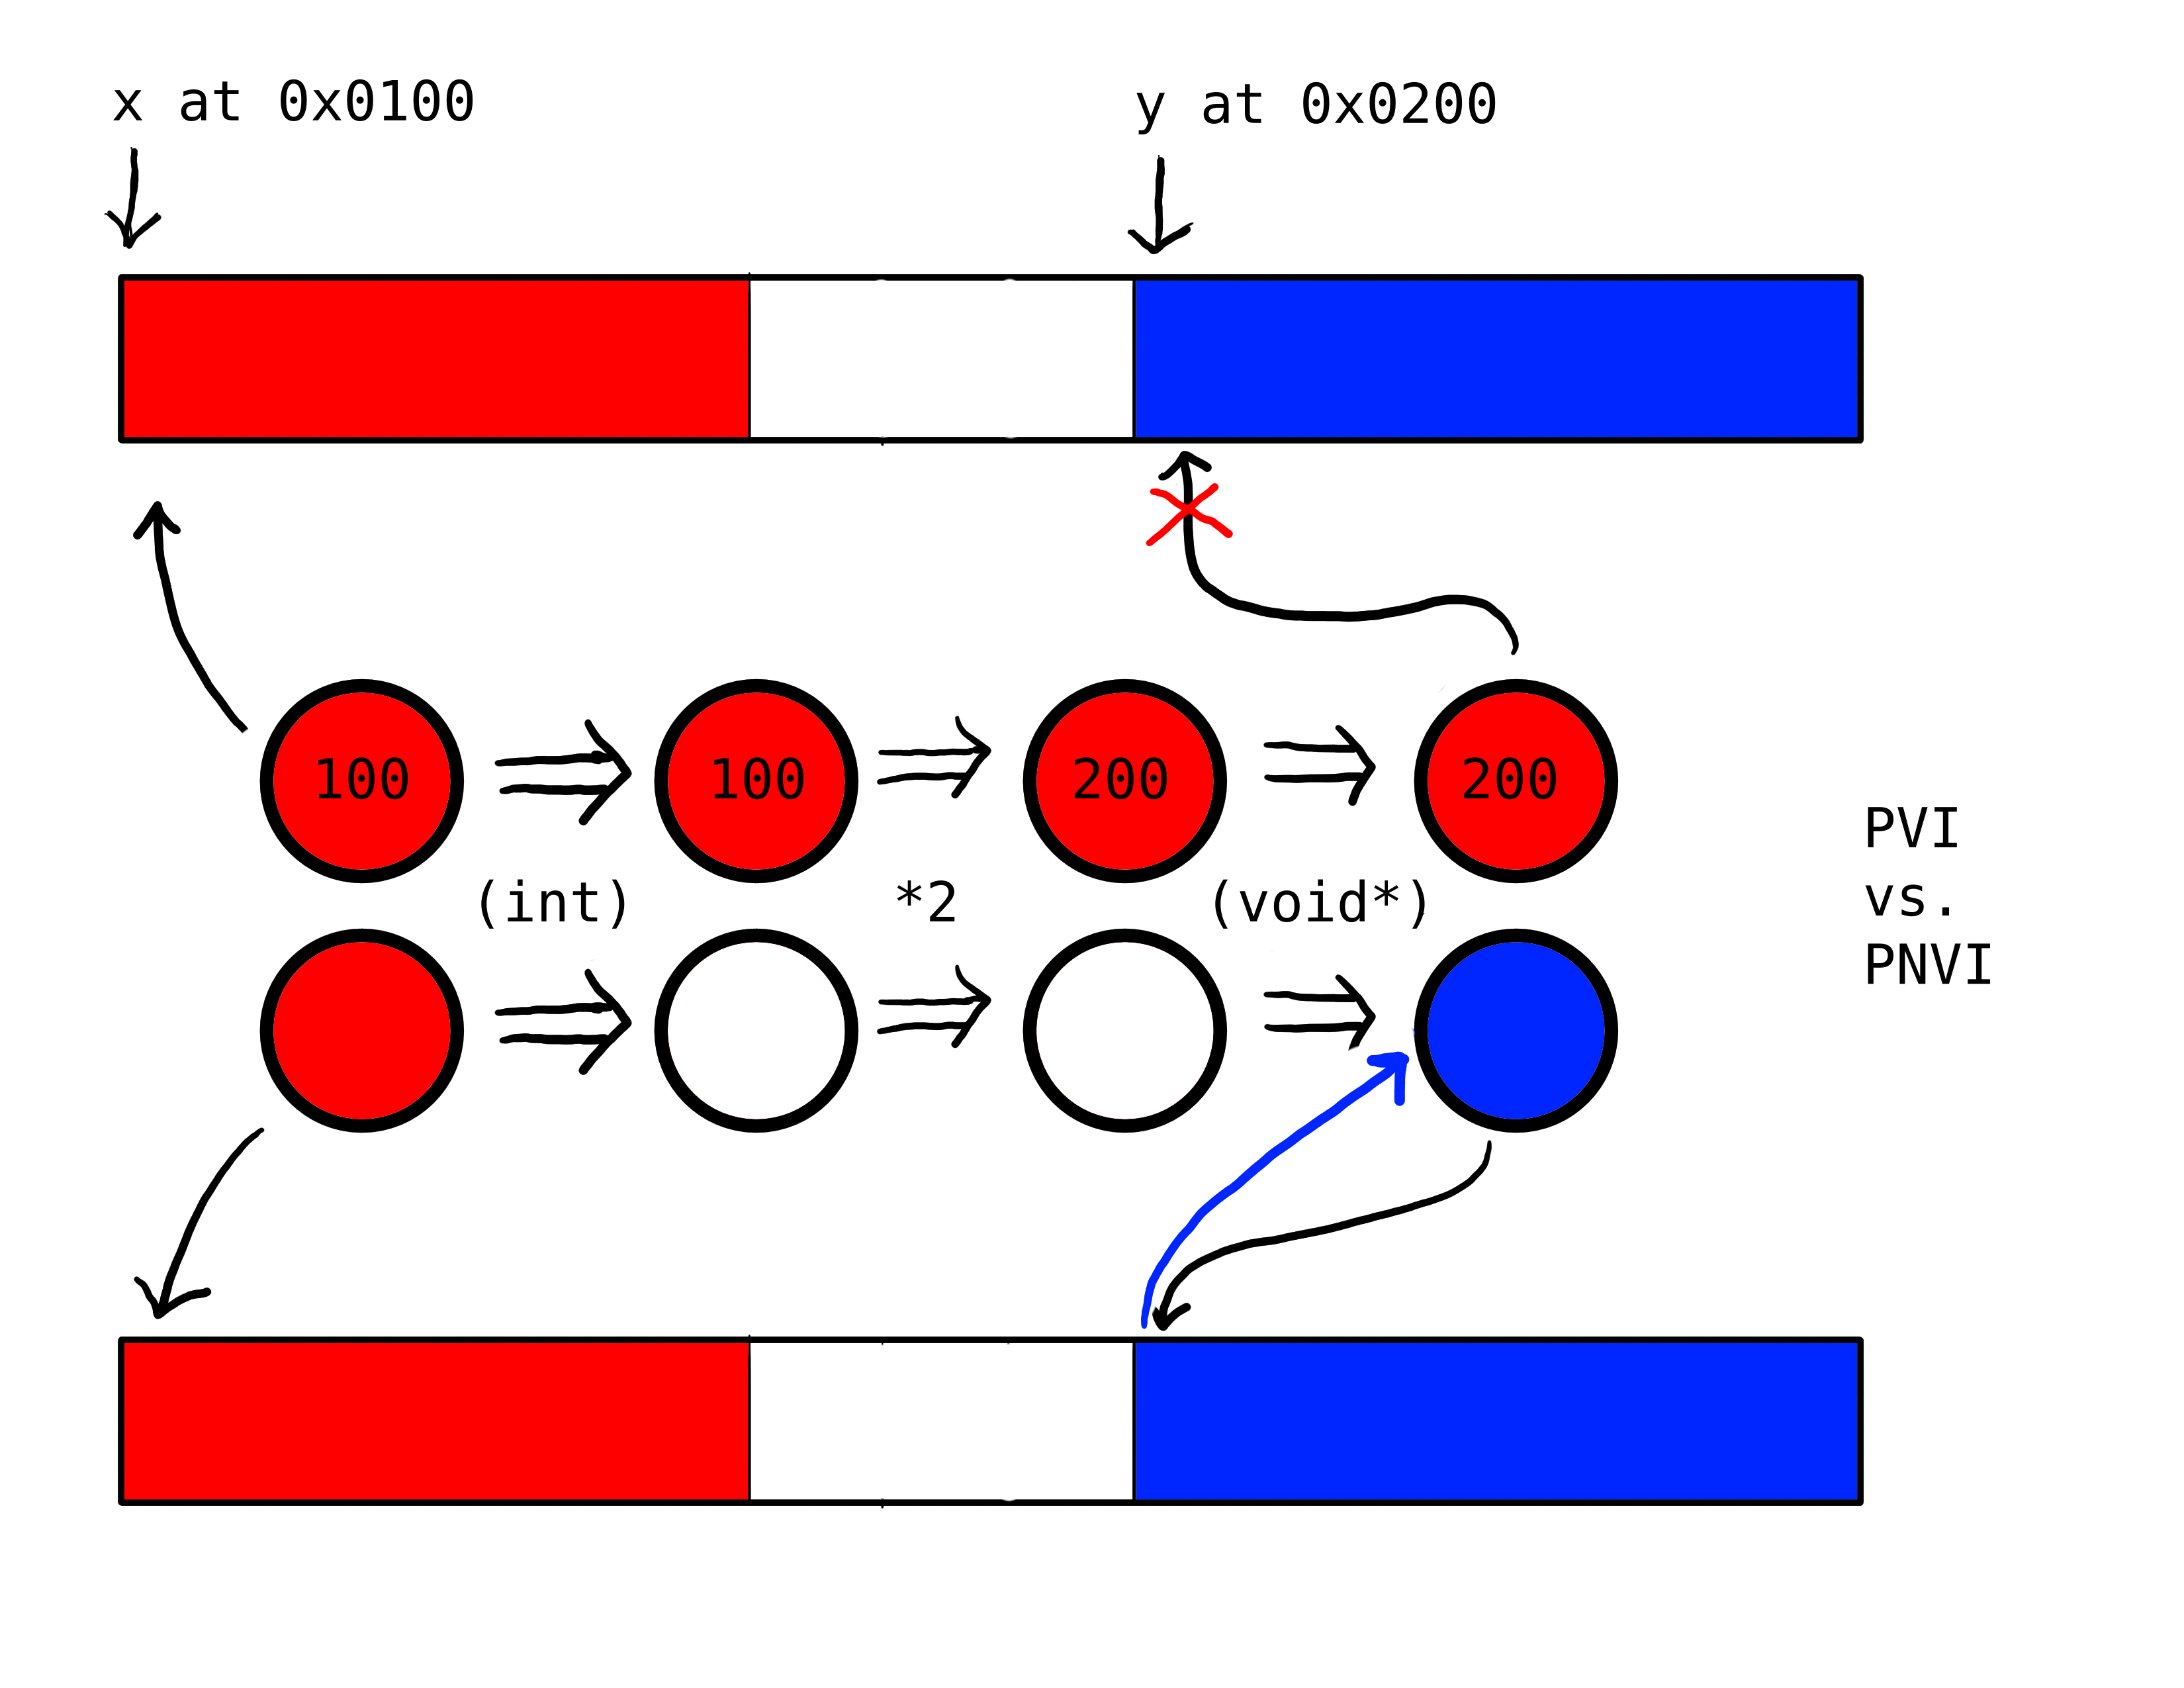
\includegraphics[width=.6\textwidth]{PVIvsPNVI.png}
%  \caption{Integer-pointer casts in PVI and PNVI}
%  \label{fig:PVI-PNVI}
%\end{figure}

%We will aim to prove that for any program, if it is run in both the PVI semantics
%and in Tagged C with our PVI policy, it either produces identical output, or it is both
%undefined in the PVI semantics and failstops in Tagged C. Likewise for PNVI, except that
%some UB in PNVI is non-deterministic, and we only require that it failstop in an execution
%that would {\it reach} the UB.

%In PNVI, the basic provenance model remains the same as PVI, so we can reuse most of the
%same rules. The primary difference is what happens when we cast a pointer to an integer.
%In PVI, tags are propagated as normal.
%To support PNVI, we need the {\it cast} expression to update the tags of a pointer
%being cast to an integer and vice versa. We add two special-case steps to reflect this.

%\judgmenttwo{\optional{\(\mem[p]_{|ty|} = \_@\vt_2 @ \overline{\lt}\)}}
%            {\(\trule{\picasttres}{\picastt}\)}
%            {\(\defestate{\cast{int}{\val{p}{\pt}}}{\tptr{ty}} \longrightarrow
%              \defestate{\val{p}{vt}}{int}\)}

%\judgmenttwo{\optional{\(\mem[p]_{|ty|} = \_@\vt_2 @ \overline{\lt}\)}}
%            {\(\trule{\ipcasttres}{\ipcastt}\)}
%            {\(\defestate{\cast{int}{\val{p}{\pt}}}{\tptr{ty}} \longrightarrow
%              \defestate{\val{p}{vt}}{int}\)}

%For casting an integer to a pointer, we don't need the optional ``peek'' at the memory that it points to.
%We simply clear the tag on the resulting integer. On the other hand, when casting back to a pointer,
%we need to check the color of the object that it points to.

%\begin{minipage}{0.34\textwidth}
%\[\begin{aligned}
%\truledef{\picastt}
%\settag{\PCT'}{\PCT}
%\settag{\vt}{N}
%\end{aligned}\]
%\end{minipage}
%\begin{minipage}{0.65\textwidth}
%\[\begin{aligned}
%\truledef{\ipcastt}
%\assert{\exists t . \forall \lt \in \overline{\lt} . \lt = t \land t \not = N}
%\settag{\PCT'}{\PCT}
%\settag{\pt}{t}
%\end{aligned}\]
%\end{minipage}

%\paragraph{Realizing the Integer-Pointer Cast}

\subsection{Secure Information Flow}
\label{sec:SIF}

Our final example policy will be a more realistic version of our first:
{\em secure information flow (SIF)}. SIF is described in the venerable Denning and Denning
\cite{Denning77:SecureInformationFlow}, and part of a larger family of policies
known as {\em information flow control} (IFC.) This family of policies deal entirely with enforcing
higher-level security concerns, regardless of whether the code that they protect contains
errors or undefined behaviors. We will give an example of a single policy in the family.
Our introductory example was an instance of {\em confidentiality}, so now we will discuss
{\em integrity}: preventing insecure input from influencing secure behavior.
In this code, a malformed user input is accidentally appended to an sql query without sanitization:

\begin{verbatim}
void sanitize(char* in, char* out);
char* sql_query(char* query);

void get_data() {
  char[20] name;
  char[20] name_san;
  char[100] query = "select address where name =";

  scanf("%19f", name);
  sanitize(name, name_san);
  strncat(query, name, strlen(name));
  
  sprintf(buf, sql_query(query));
  return;
}
\end{verbatim}

This function sanitizes its input {\tt name}, then appends the result to an appropriate SQL
query, storing the result in {\tt buf}. But, in the default case, the programmer has accidentally
used the unsanitized string! This creates the opportunity for an SQL injection attack: a caller
to this function could (presumably at the behest of an outside user) call it with {\tt field} of
3 and {\tt name} of ``Bobby; drop table;''.

The fact that the input can be sanitized also makes this an {\em intransitive} policy:
information may flow from {\tt scanf} to {\tt sanitize}, and from {\tt sanitize} to
{\tt sql\_query}, but not directly from {\tt scanf} to {\tt sql\_query}.

\begin{figure}

  \begin{minipage}{0.3\textwidth}
    \color{blue}
    \begin{align*}
      \tau ::= & \high \\
      & \low \\
      & \pctaint{f}{e}{\overline{L}} & e \in \mathit{list} ~ \mathbb{B} \\
    \end{align*}
  \end{minipage}
  \begin{minipage}{0.69\textwidth}
    \[|\gentag| \triangleq
    \begin{cases}
      \low & \textnormal{if } \gentag = \low \textnormal{ or } \gentag = \pctaint{f}{e}{\emptyset}
      \textnormal{ where every } b \in e \textnormal{ is } \mathbf{f} \\
      \high & \textnormal{otherwise} \\
    \end{cases}\]
    %
    \[\gentag_1 \sqcup \gentag_2 \triangleq
    \begin{cases}
      \low & \textnormal{if } |\gentag_1| = |\gentag_2| = \low \\
      \high & \textnormal{otherwise} \\
    \end{cases}\]
  \end{minipage}

  \begin{minipage}{0.54\textwidth}
    \storetruleblock
        {let \(\pctaint{f}{ets}{\overline{L}} := \PCT\) in \\
          \caseofthree{\(f\)}
                      {\(\mathit{scanf}\)}{\high}
                      {\(\mathit{sanitize}\)}{\low}
                      {\(\underline{\hspace{3em}}\)}
                      {\(\PCT' := \PCT\) \\
                        \(\vt' := \PCT \sqcup \vt \sqcup \pt\) \\
                        \(\lts' := \lts\)}}
  \end{minipage}
  \begin{minipage}{0.45\textwidth}
    \loadtruleblock
        {let \(\pctaint{f}{ets}{\overline{L}} := \PCT\) in \\
          \caseoftwo{\(f\)}
                    {\(\mathit{sql\_query}\)}{\(\mathbf{assert} ~ \vt \sqcup \pt = \low\) \\ & & \(\vt' := \vt\)}
                    {\(\underline{\hspace{3em}}\)}{\(\vt' := \vt\)}}

    \binoptruleblock{\(\vt' := \vt_1 \sqcup \vt_2\)}
  \end{minipage}

\caption{SIF Policy: Tags and Selected Rules}
\label{fig:sif1}
\end{figure}

Since we care about a single source, we can once again use the standard division of \(\high\)
and \(\low\). We additionally need to carry significant information on the PC Tag. First, we
track the current function identifier. Beyond that, we need two pieces of information to deal
with {\em implicit flows}, situations where the control-flow of the program is influenced by a secret.
In our initial example we simplified these. To keep track of tainted scopes, the
PC Tag carries a list of booleans, \(e\), and a set of label identifiers, \(L\).
We will discuss these in detail below. Initially, the PC Tag is \(\pctaint{f}{\varepsilon}{\emptyset}\),
and all values and memory locations are tagged \(\low\).

The detailed tag rules for expressions are given in \cref{fig:sif1}. We define two operators on tags:
the ``join'' operator \(\sqcup\) takes the higher of two security levels, and the ``reduce''
operator \(| \cdot |\) converts a PC Tag into a security level, \(\high\) or \(\low\).
The function {\tt scanf} taints all of its writes by marking them \(\high\). This extends to
its return value in \(\rettname\) as well (not shown.) By the same token, all outputs of
{\tt sanitize} are tagged \(\low\), so that when it copies \(\high\)-tagged data into its
output buffer, we consider those data safe.

In this scenario, our policy aims to prevent {\tt sql\_query} from recieving tainted data.
For this reason, we failstop if {\tt sql\_query} would load a tainted value.

\paragraph*{Implicit Flows}

\begin{figure}[t]
  \begin{subfigure}{0.49\textwidth}
\begin{verbatim}
int f(bool secret) {
    int public1, public2;

S:  if (secret) {
b1:     public1 = 1;
    } else {
b2:     public1 = 0;
    }

J:  public2 = 42;
    return public2;
}
\end{verbatim}
  \end{subfigure}
  \begin{subfigure}{0.5\textwidth}
    \begin{tikzpicture}
      [ initial text={}, initial distance=4em,
        accepting/.style=accepting by arrow,
        accepting distance=4em
      ]
      \node[state,initial]    (S)                        {$S$};
      \node[state]            (b_1) [above right=of S]   {$b_1$};
      \node[state]            (b_2) [below right=of S]   {$b_2$};
      \node[state,accepting]  (J)   [below right=of b_1] {$J$};

      \path[->] (S)   edge              node  {}  (b_1)
                      edge              node  {}  (b_2)
                (b_1) edge              node  {}  (J)
                (b_2) edge              node  {}  (J);
    \end{tikzpicture}
  \end{subfigure}
\caption{Leaking via if statements}
\label{fig:ifthenelse}  
\end{figure}

Things become trickier when we consider that the program's control-flow itself can be tainted.
This can occur in any conditional, including loops, conditional statements, and conditional expressions.
In general, anytime a ``split'' is conditioned on a tainted value, subsequent assignments must also be tainted.
An example can be seen in \cref{fig:ifthenelse}, where labels in the code indicate the split
point, branches, and {\em join point} \(J\).

A join point is the node in the program's control-flow graph where all possible routes
from the split to a return have re-converged; its its immediate post-dominator \cite{}.
[TODO: this is the Denning cited in Bay and Askarov] At this point, an observer can no
longer deduce which path execution took, except through the assignments that happened
in \(b_1\) or \(b_2\), which are already tainted. It is therefore safe to tag future
assignments \(\low\). In the example, {\tt public1} should be tagged \(\high\), while
{\tt public2} is tagged \(\low\).

We assume a {\em termination-insensitive} setting \cite{Askarov08:TINILeaks}, in which
we allow an observer to glean information by the termination or non-termination of
the program. This is a necessary limitation of an enforcement mechanism that halts
execution. Having accepted this limitation, we may apply the same analysis to loops
as well as conditionals.

\Cref{fig:SIFconditionals} gives the tag rules for handling conditionals and loops.
All branching statements are governed by the same \(\splittname\) rule, and their join points
by the \(\labeltname\) rule when the label is placed on a join point. Branching expressions
are likewise handled by the \(\exprsplittname\) rule, and the \(\exprjointname\) rule.
This last needs no label, due to the predictable structure of nested expressions.

\begin{figure}
  \begin{minipage}{0.5\textwidth}
    \splittruleblock{
      let \(\pctaint{f}{e}{\overline{L}} := \PCT\) in \\
      \caseoftwo{\(\vt\)}
                {\(\high\)}{\(\PCT' := \pctaint{f}{e}{(L \cup \overline{L})}\)}
                {\(\low\)}{\(\PCT' := \PCT\)}
    }
    \labeltruleblock{
      let \(\pctaint{f}{e}{\overline{L}} := \PCT\) in \\
      \(\PCT' := \pctaint{f}{e}{\overline{L} - L}\)
    }
  \end{minipage}
  \begin{minipage}{0.49\textwidth}
    \exprsplittruleblock{
      let \(\pctaint{f}{e}{\overline{L}} := \PCT\) in \\
      \caseoftwo{\(\vt\)}
                {\(\high\)}{\(\PCT' := \pctaint{f}{\mathbf{t}::e}{\overline{L})}\)}
                {\(\low\)}{\(\PCT' := \pctaint{f}{(\mathbf{f}::e}{\overline{L})}\)}
    }

    \exprjointruleblock{
      let \(\pctaint{f}{b::e}{\overline{L}} := \PCT\) in \\
      \(\PCT' := \pctaint{f}{e}{\overline{L}}\)
    }
  \end{minipage}
  
  \caption{SIF Conditionals}
  \label{fig:SIFconditional Rules}
\end{figure}

Of course, code does not generally come with labeled join points, and they must be associated
with their split points. We introduce additional forms of the if, while, do-while, for, and switch
statements which carry an additional label, and perform some preprocessing to associate these
with new labels in the source code. This preprocessing step generates the program's
control flow graph and, for each branch, identifies its immediate post-dominator. That
node is labeled with  a fresh identifier, and the same identifier is added to the original
conditional statement.

%\begin{figure}
%  \begin{subfigure}{0.49\textwidth}
%\begin{verbatim}
%int f(bool secret) {
%    int public1=1;
%    int public2;
%
%S:  while (secret) {
%b1:     public1 = 1;
%        secret = false;
%    }
%
%J:  public2 = 42;
%
%    return public2;
%}
%\end{verbatim}
%  \caption{Leaking via while statements}
%  \label{fig:while}
%  \end{subfigure}
%  \begin{subfigure}{0.5\textwidth}
%    \begin{tikzpicture}
%      [ initial text={}, initial distance=4em,
%        accepting/.style=accepting by arrow,
%        accepting distance=4em
%      ]
%      \node[state,initial]    (S)                        {$S$};
%      \node[state]            (b_1) [above right=of S]   {$b_1$};
%      \node[state,accepting]  (J)   [below right=of b_1] {$J$};

%      \path[->] (S)   edge               node  {}  (b_1)
%                      edge               node  {}  (J)
%                (b_1) edge [bend right] node  {}  (S);
%    \end{tikzpicture}
%  \end{subfigure}
%  
%\end{figure}

%\begin{figure}
%  \begin{subfigure}{0.25\textwidth}
%\begin{verbatim}
%int f(bool secret) {
%    int public1, public2;

%    while (secret) {
%        goto b1;
%    }

%b2: public1 = 1;
%    goto J;

%b1: public1 = 1;

%J:  public2 = 42;
%    return public2;
%}
%\end{verbatim}
%  \end{subfigure}
%  \begin{subfigure}{0.74\textwidth}
%    \begin{tikzpicture}
%      [ initial text={}, initial distance=3em,
%        accepting/.style=accepting by arrow,
%        accepting distance=3em
%      ]
%      \node[state,initial]    (S)                              {$S$};
%      \node[state]            (inside) [above right=of S]      {};
%      \node[state]            (b_2)    [below right=of inside] {$b_2$};
%      \node[state]            (b_1)    [right=of b_2]          {$b_1$};
%      \node[state,accepting]  (J)      [right=of b_1]          {$J$};

%      \path[->] (S)   edge              node  {}  (inside)
%                      edge              node  {}  (b_2)
%                (inside) edge [bend left] node {} (b_1)
%                (b_1) edge              node  {}  (J)
%                (b_2) edge [bend right] node  {}  (J);
%    \end{tikzpicture}
%  \end{subfigure}
  
%  \caption{Cheating with go-tos}
%  \label{fig:forbreak}
%\end{figure}
%\begin{figure}
%  \begin{subfigure}{0.3\textwidth}
%    \begin{tikzpicture}
%      [ initial text={}, initial distance=1em,
%        accepting/.style=accepting by arrow,
%        accepting distance=1em
%      ]
%      \node[state,initial]    (do)                             {do};
%      \node[state,accepting]  (S) [right=of do]                {\(S\):test};

%      \path[->] (do)   edge              node  {}  (S)
%                (S)    edge [bend left]  node  {}  (do);
%    \end{tikzpicture}
%    \subcaption{Do-while}
%  \end{subfigure}
%  \begin{subfigure}{0.3\textwidth}
%    \begin{tikzpicture}
%      [ initial text={}, initial distance=1em,
%        accepting/.style=accepting by arrow,
%        accepting distance=1em
%      ]
%      \node[state,initial]    (init)                             {init};
%      \node[state,accepting]  (S)    [right=of init]             {\(S\):test};
%      \node[state]            (do)   [above=of S]                {do};
%      \node[state]            (post) [left=of do]                {post};
      
%      \path[->] (init)   edge              node  {}  (S)
%                (S)      edge              node  {}  (do)
%                (do)     edge              node  {}  (post)
%                (post)   edge              node  {}  (S);
%    \end{tikzpicture}
%    \subcaption{For}
%  \end{subfigure}
%  \begin{subfigure}{0.3\textwidth}
%    \center
%    \begin{tikzpicture}
%      [ initial text={}, initial distance=1em, initial above,
%        accepting/.style=accepting by arrow,
%        accepting distance=1em, node distance=2em, inner sep=1pt
%      ]
%      \node[state,initial]    (switch)                           {\(S\):switch};
%      \node[state]            (case1)    [below left=of switch]  {};
%      \node[state]            (case2)    [right=of case1]        {};
%      \node[state]            (default)  [right=of case2]        {def};
%      \node                   (after)    [right=of default]      {};

%      \path[->] (switch)  edge              node  {}  (case1)
%                          edge              node  {}  (case2)
%                          edge              node  {}  (default)
%                (default) edge              node  {}  (after)
%                (case1)   edge [bend right] node  {}  (after)
%                (case2)   edge [bend right] node  {}  (after);

%      \path[dotted,->] (case1) edge              node  {}  (case2)
%                (case2) edge              node  {}  (default);
                         
%    \end{tikzpicture}
%    \subcaption{Switch}
%  \end{subfigure}
  
%  \caption{Remaining Branch Statements}
%  \label{fig:rest}
%\end{figure}


\section{Implementing Tagged C with PIPE}
\label{sec:optionals}

Chhak et al. \cite{Chhak21:Tagine} introduce a verified compiler from a toy
high-level language with tags
to a control-flow-graph-based intermediate representation of a PIPE-based
ISA. It is a proof-of-concept of compilation from a source language's tag policy to
realistic hardware. Everything in a PIPE system carries tags, including instructions. 
Instruction tags are statically determined at compile-time, so they can carry data about source-level
control points in the corresponding assembly. This means that PIPE can emulate any given Tagged C
policy by running two policies in parallel: a basic stack-and-function-pointer-safety policy to mimic Tagged C's
high-level control-flow, and the source-level policy as written.

Chhak et al.'s general strategy for mapping Tagged C's tag rules sometimes requires adding extra
instructions to the generated code. A Tagged-C control point
may require a tag from a location that is not read under a normal compilation scheme, or must update tags
in locations that would otherwise not be written. Such instructions are unnecessary overhead if the policy
doesn't meaningfully use the relevant tags.

To mitigate this, control points whose compilation would add potentially extraneous instructions
take optional parameters or return optional results. We will explain how the rule should be
implemented in the target if the options are used.
\sna{I think we have been leaning toward doing so in more detail here, not threaded through the
  rest of the paper. So that's a TODO.}
Optional inputs and outputs are marked with \(\optional{boxes}\). If a policy does not make use of the options, it will
be sound to compile without the extra instructions.

\section{Evaluation}
\label{sec:evaluation}

Tagged C aims to combine the flexibility of tag-based architectures with the abstraction
of a high-level language. How well have we achieved this aim?

[Here we list criteria and evaluate how we fulfilled them]

\begin{itemize}
\item Flexibility: we demonstrate three policies that can be used alone or in conjunction
\item Applicability: we support the full complement of C language features and give definition
  to many undefined C programs
\item Practical security: our example security policies are based on important security concepts
  from the literature
\end{itemize}

\subsection{Limitations of the Tag Mechanism}

By committing to a tag-based mechanism, we do restrict the space of policies that Tagged C
can enforce. In general, a reference monitor can enforce any policy that constitutes a
{\em safety property}---any policy whose violation can be demonstrated by a single finite
trace. This class includes such policies as ``no integer overflow'' and ``pointers are always in-bounds,''
which depend on the values of variables. Tag-based monitors cannot enforce any policy that
depends on the value of a variable rather than its tags.

\section{Related Work}

\paragraph{Reference Monitors}

The concept of a reference monitor was first introduced fifty years ago in \cite{Anderson72:PlanningStudy}:
a tamper-proof and verifiable subsystem that checks every security-relevant operation in a system to
ensure that it conforms to a security {\em policy} (a general specification of acceptable behavior;
see \cite{Goguen82:SecurityPolicies}.)

A reference monitor can be implemented at any level of a system. An {\em inline reference monitor}
is a purely compiler-based system that inserts checks at appropriate places in the code.
Alternatively, a reference monitor might be embedded in the operating system, or in an interpreted
language's runtime. A {\em hardware reference monitor} instead provides primitives at the ISA-level
that accelerate security and make it harder to subvert.

Programmable Interlocks for Policy Enforcement (PIPE) \cite{Dhawan14:PUMP} is a hardware extension
that uses {\em metadata tagging}. Each register and each word of memory is associated with
an additional array of bits called a tag. The policy is decomposed into a set of {\em tag rules}
that act in parallel with each executing instruction, using the tags on its operands to
decide whether the instruction is legal and, if so, determine which tags to place on its results.
PIPE tags are large relative to other tag-based hardware, giving it the flexibility
to implement complex policies with structured tags, and even run multiple policies at once.

Other hardware monitors include Arm MTE, [Binghamton], and CHERI.
Arm MTE aims to enforce a narrow form of memory safety using 4-bit tags, which distinguish adjacent objects
in memory from one another, preventing buffer overflows, but not necessarily other memory violations.
[TODO: read the Binghamton paper, figure out where they sit here.] 

CHERI is capability machine [TODO: cite OG CHERI]. In CHERI, capabilities
are ``fat pointers'' carrying extra bounds and permission information, and capability-protected
memory can only be accessed via a capability with the appropriate privilege. This is a natural
way to enforce spatial memory safety, and techniques have been demonstrated for enforcing
temporal safety \cite{NWF20:Cornucopia}, stack safety \cite{Skorstengaard19:stktokens},
and compartmentalization [TODO: figure out what to cite], with varying degrees of ease and
efficiency. But CHERI cannot easily enforce notions of security based on dataflow,
such as Secure Information Flow.

In this paper, we describe a programming language with an abstract reference monitor.
We realize it as an interpreter with the reference monitor built in, and envision
eventually compiling to PIPE-equipped hardware. An inlining compiler would also be plausible.
As a result of this choice, our abstract reference monitor uses a PIPE-esque notion of
tags.

\paragraph{Aspect Oriented Programming}

[TODO: do forward search from original AOP paper]

\section{Future Work}
\label{sec:futurework}

We have presented the language and a reference interpreter, built on top of the CompCert interpreter
\cite{Leroy09:CompCert}, and three example policies. There are several significant next-steps.

\paragraph{Compilation}

An interpreter is all well and good, but a compiler would be preferable for many reasons.
A compiled Tagged C could use the hardware acceleration of a PIPE target, and could more easily
support linked libraries, including linking against code written in other languages.
The ultimate goal would be a fully verified compiler, but that is a very long way off.

\paragraph{Language Proofs}

There are a couple of properties of the language semantics itself that we would like to prove.
Namely (1) that its behavior (prior to adding a policy) matches that of CompCert C and
(2) that the behavior of a given program is invariant under all policies up to truncation due
to failstop.

\paragraph{Policy Correctness Proofs}

For each example policy discussed in this paper, we sketched a formal specification for the
security property it ought to enforce. A natural continuation would be to prove the correctness
of each policy against these specifications.

\paragraph{Policy DSL}

Currently, policies are written in Gallina, the language embedded in Coq. This is fine for a
proof-of-concept, but not satisfactory for real use. We plan to develop a domain-specific policy
language to make it easier to write Tagged C policies.

\bibliographystyle{splncs04}
\bibliography{taggedc.bib}

\appendix

\section{Syntax}

\begin{figure}
  \begin{subfigure}[t]{0.3\textwidth}
    \[\begin{aligned}
    \stmt ::= & \sskip \\
    | & \sdo{\expr} \\
    | & \sseq{\stmt_1}{\stmt_2} \\
    | & \sifthenelse{\expr}{\stmt_1}{\stmt_2}{L} \\
    | & \swhile{\expr}{\stmt}{L} \\
    | & \sdowhile{\expr}{\stmt}{L} \\
    | & \sfor{\stmt_1}{\expr}{\stmt_2}{\stmt_3} \\
    | & \sbreak \\
    | & \scontinue \\
    | & \sreturn \\
    | & \sswitch{\expr}{\overline{(L,\stmt)}} \\
    | & \slabel{L}{\stmt} \\
    | & \sgoto{L} \\    
    \end{aligned}\]
  \end{subfigure}
  \begin{subfigure}[t]{0.69\textwidth}
    \[\begin{aligned}
    \expr ::= & \val{v}{\vt} & \textnormal{Value} \\
    | & \var{x} & \textnormal{Variable} \\
    | & \field{\expr}{id} & \textnormal{Field} \\
    | & \valof{\expr} & \textnormal{Load from Object} \\
    | & \deref{\expr} & \textnormal{Dereference Pointer} \\
    | & \addrof{\expr} & \textnormal{Address of Object} \\
    | & \unop{\odot}{\expr} & \textnormal{Unary Operator} \\
    | & \binop{\oplus}{\expr_1}{\expr_2} & \textnormal{Binary Operator} \\
    | & \cast{\expr}{ty} & \textnormal{Cast} \\
    | & \condition{\expr_1}{\expr_2}{\expr_3} & \textnormal{Conditional} \\
    | & \sizeof{ty} & \textnormal{Size of Type} \\
    | & \alignof{ty} & \textnormal{Alignment of Type} \\
    | & \assign{\expr_1}{\expr_2} & \textnormal{Assignment} \\
    | & \assignop{\oplus}{\expr_1}{\expr_2} & \textnormal{Operator Assignment} \\
    | & \postinc{\oplus}{\expr} & \textnormal{Post-Increment/Decrement} \\
    | & \comma{\expr_1}{\expr_2} & \textnormal{Expression Sequence} \\
    | & \call{\expr_f}{\overline{\expr}_{args}} & \textnormal{Function Call} \\
    | & \loc{l}{\lt} & \textnormal{Memory Location} \\
    | & \paren{\expr}{ty}{\gentag} & \textnormal{Parenthetical with Optional Cast} \\
    \end{aligned}\]
  \end{subfigure}
  \caption{Tagged C Abstract Syntax}
  \label{fig:syntax}
\end{figure}

\section{Continuations}
\label{app:continuations}

\[\begin{split}
\cont ::= & \kemp \\
| & \kdo{\cont} \\
| & \kseq{\stmt}{\cont} \\
| & \kif{\stmt_1}{\stmt_2}{L}{\cont} \\
| & \kwhiletest{\expr}{\stmt}{L}{\cont} \\
| & \kwhileloop{\expr}{\stmt}{L}{\cont} \\
| & \kdowhiletest{\expr}{\stmt}{L}{\cont} \\
| & \kdowhileloop{\expr}{\stmt}{L}{\cont} \\
| & \kfor{\expr}{\stmt_2}{\stmt_3}{L}{\cont} \\
| & \kforpost{\expr}{\stmt_2}{\stmt_3}{L}{\cont} \\
\end{split}\]

\section{States}

States can be of several kinds, denoted by their script prefix: a {\em general state} \(\mathcal{S}(\dots)\),
an {\em expression state} \(\mathcal{E}(\dots)\), a {\em call state} \(\mathcal{C}(\dots)\), or a
{\em return state} \(\mathcal{R}(\dots)\). Finally, the special state {\em failstop} (\(\mathcal{F}(\dots)\))
represents a tag failure, and carries the state that produced the failure.
[Allison: to whatever degree you've figured out what is useful here by publication-time, we can
  tune this to be more specific.]

\[\begin{aligned}
S ::= & \sstate{\PCT}{\mem}{\stmt}{\cont} \\
| & \estate{\PCT}{\mem}{\expr}{\cont} \\
| & \cstate{f}{\PCT}{\mem}{\lenv}{f'}{\overline{\val{v}{\vt}}}{\cont} \\
| & \rstate{\PCT}{\mem}{\genv}{\lenv}{\val{v}{\vt}}{\cont} \\
| & \fstate{S} \\
\end{aligned}\]

\section{Initial State}

Given a list \(xs\) of variable identifiers \(id\) and types
\(ty\), a program's initial memory is defined by iteratively allocating each one
in memory and updating the global environment with its base address, bound, type,
and a static identity tag. Let \(|ty|\) be a function from types to their sizes
in bytes. The memory is initialized \(\vundef@\vt@\overline{\lt}\)
for some \(\vt\) and \(\overline{\lt}\), unless given an initializer.
Let \(\mem_0\) and \(\genv_0\) be the initial (empty) memory and environment.
The parameter \(b\) marks the start of the global region.

%Since we don't need to initialize tags in memory dynamically, our rule for
%selecting these tags can cover the entire initialization of the memory with arbitrary
%granularity. We represent this as a list of tags of length \(|ty|\).

\[\mathit{globals} ~ xs ~ b =
\begin{cases}
  (\mem_0, \genv_0) & \textnormal{if } xs = \varepsilon \\
  (\mem[p \dots p+|ty| \mapsto \vundef@\vt@\overline{\lt}]_{|ty|}, & \textnormal{if } xs = (id,ty)::xs' \\
  ~ \genv[id \mapsto (\mathit{p, p+|ty|,ty,\pt})]) & \textnormal{and } \trule{\globaltres}{\globalt} \\
  & \textnormal{where } (\mem,\genv) = \mathit{globals} ~ xs' ~ (b + |ty|) \\
\end{cases}\]

\section{Step Rules}
\label{app:rules}

\subsection{Sequencing rules}

\sequencing

\subsection{Conditional rules}

\conditionals

\subsection{Loop rules}

\loops

\subsection{Contexts}
\label{app:contexts}

Our expression semantics are contextual. A context \(\mathit{ctx}\) is a function from an
expression to an expression and a tag. We identify a valid context using the \(\mathit{context}\)
relation over a ``kind'' (left-hand or right-hand, \(\lh\) or \(\rh\)),
and an expression.

\[\begin{aligned}
\mathit{context} & ~ k ~ \ctx{\expr} ::= \\
| & \mathit{context} ~ k ~ \lambda \expr.\expr & \\ % ctx_top
| & \mathit{context} ~ \lh ~ \lambda \expr.\deref{\ctx{\expr}} &
\textnormal{where } \mathit{context} ~  \rh ~ \ctx{\expr} \\ % ctx_deref
| & \mathit{context} ~ \lh ~ \lambda \expr.\field{\ctx{\expr}}{id} &
\textnormal{where } \mathit{context} ~  \rh ~ \ctx{\expr} \\ % ctx_field
| & \mathit{context} ~ \rh ~ \lambda \expr.\valof{\ctx{\expr}} &
\textnormal{where } \mathit{context} ~  \lh ~ \ctx{\expr} \\ % ctx_rvalof
| & \mathit{context} ~ \rh ~ \lambda \expr.\addrof{\ctx{\expr}} & \textnormal{where } \mathit{context} ~  \lh ~ \ctx{\expr} \\ % ctx_addrof
| & \mathit{context} ~ \rh ~ \lambda \expr.\unop{\odot}{\ctx{\expr}} & \textnormal{where } \mathit{context} ~  \rh ~ \ctx{\expr} \\ % ctx_unop
| & \mathit{context} ~ \rh ~ \lambda \expr.\binop{\oplus}{\ctx{\expr_1}}{\expr_2} & \textnormal{where } \mathit{context} ~  \rh ~ \ctx{\expr_1} \\ % ctx_binop_left
| & \mathit{context} ~ \rh ~ \lambda \expr.\binop{\oplus}{\expr_1}{\ctx{\expr_2}} & \textnormal{where } \mathit{context} ~  \rh ~ \ctx{\expr_2} \\ % ctx_binop_right
| & \mathit{context} ~ \rh ~ \lambda \expr.\cast{\ctx{\expr}}{\type} & \textnormal{where } \mathit{context} ~  \rh ~ \ctx{\expr} \\ % ctx_cast
| & \mathit{context} ~ \rh ~ \lambda \expr.\seqand{\ctx{\expr_1}}{\expr_2} & \textnormal{where } \mathit{context} ~  \rh ~ \ctx{\expr_1} \\ % ctx_seqand
| & \mathit{context} ~ \rh ~ \lambda \expr.\seqor{\ctx{\expr_1}}{\expr_2} & \textnormal{where } \mathit{context} ~  \rh ~ \ctx{\expr_1} \\ % ctx_seqor
| & \mathit{context} ~ \rh ~ \lambda \expr.\condition{\ctx{\expr_1}}{\expr_2}{\expr_3} & \textnormal{where } \mathit{context} ~  \rh ~ \ctx{\expr_1} \\ % ctx_condition
| & \mathit{context} ~ \rh ~ \lambda \expr.\assign{\ctx{\expr_1}}{\expr_2} & \textnormal{where } \mathit{context} ~  \lh ~ \ctx{\expr_1} \\ % ctx_assign_left
| & \mathit{context} ~ \rh ~ \lambda \expr.\assign{\expr_1}{\ctx{\expr_2}} & \textnormal{where } \mathit{context} ~  \rh ~ \ctx{\expr_2} \\ % ctx_assign_right
| & \mathit{context} ~ \rh ~ \lambda \expr.\assignop{\oplus}{\ctx{\expr_1}}{\expr_2} & \textnormal{where } \mathit{context} ~ \lh ~ \ctx{\expr_1} \\ % ctx_assignop_left
| & \mathit{context} ~ \rh ~ \lambda \expr.\assignop{\oplus}{\expr_1}{\ctx{\expr_2}} & \textnormal{where } \mathit{context} ~ \rh ~ \ctx{\expr_2} \\ % ctx_assignop_right
| & \mathit{context} ~ \rh ~ \lambda \expr.\postinc{\oplus}{\ctx{\expr}} & \textnormal{where } \mathit{context} ~  \lh ~ \ctx{\expr} \\ % ctx_postinc
| & \mathit{context} ~ \rh ~ \lambda \expr.\call{\ctx{\expr_1}}{\overline{\expr_2}} & \textnormal{where } \mathit{context} ~  \rh ~ \ctx{\expr_1} \\ % ctx_call_left
| & \mathit{context} ~ \rh ~ \lambda \expr.\call{\expr_1}{\ctx{\overline{\expr_2}}} & \textnormal{where } \mathit{context} ~  \rh ~ \ctx{\expr} \textnormal{ for } \expr \in \overline{\expr_2} \\ % ctx_call_right
% skipped builtins
| & \mathit{context} ~ \rh ~ \lambda \expr.\comma{\ctx{\expr_1}}{\expr_2} & \textnormal{where } \mathit{context} ~  \rh ~ \ctx{\expr_1} \\ % ctx_comma
| & \mathit{context} ~ \rh ~ \lambda \expr.\paren{\ctx{\expr}}{\type}{} & \textnormal{where } \mathit{context} ~  \rh ~ \ctx{\expr} \\ % ctx_paren
| & \mathit{context} ~ \rh ~ \lambda \expr.\paren{\ctx{\expr}}{\type}{\gentag} & \textnormal{where } \mathit{context} ~ \rh ~ \ctx{\expr} \\ % ctx_paren
\end{aligned}\]

Next, we define a notion of expression reduction. A left-hand reduction relates an expression to an expression.
A right-hand reduction relates a triple of PC Tag, memory, and expression to another such triple.

%triple of a memory, an expression, and a tag
%might reduces to another such triple as a left-hand, right-hand, or call reduction, written
%\((\mem, \expr, \PCT) \Rightarrow_k (\mem', \expr', \PCT')\),
%based on rules given below. These reductions are embedded in states as follows.

\judgmenttwo{\(\mathit{context} ~ \lh ~ \ctx{\expr}\)}
            {\(\expr \Rightarrow_\lh \expr'\)}
            {\(\defestate{\ctx{\expr}} \longrightarrow \defestate{\ctx{\expr}}\)}

\judgmenttwo{\(\mathit{context} ~ \rh ~ \ctx{\expr}\)}
            {\((\PCT, \mem, \expr) \Rightarrow_\rh (\PCT', \mem', \expr')\)}
            {\(\defestate{\ctx{\expr}} \longrightarrow \estate{\PCT'}{\mem'}{\ctx{\expr}}{\cont}\)}
            
\subsection{Expression Rules}

\expressions

\subsection{Call and Return Rules}

In order to make a call, we need to reduce the function expression to an \(\floc{\_}\) value, an
abstract location corresponding to a particular function. Then we can make the call.

\callexprstep

When we make an internal call, we need to allocated space for locals and arguments using the helper function
\(\mathit{frame}\).

\[\mathit{frame} ~ xs ~ as ~ \mem =
\begin{cases}
  (\mem''[p \mapsto \vundef@\vt@\overline{\lt}]_{|ty|}, & \textnormal{if } xs = (id,ty)::xs' \\
  \lenv'[id \mapsto (\mathit{p, p+|ty|,ty,\pt})]) &
  \textnormal{where } (\mem',p) \leftarrow \mathit{stack\_alloc} ~ |ty| ~ \mem, \\
  & \trule{\localtres}{\localt}, \\
  & \textnormal{and } (\mem'',\lenv') = \mathit{frame} ~ xs' ~ as ~ m' \\ 
  \\
  (\mem''[p \mapsto v@\vt'@\overline{\lt}]_{|ty|}, & \textnormal{if } as = (id,ty,v @ \vt)::as' \textnormal{ and } xs = \varepsilon \\
  \lenv'[id \mapsto (\mathit{p, p+|ty|,ty,\pt})]) &
  \textnormal{where } (\mem',p) \leftarrow \mathit{stack\_alloc} ~ |ty| ~ \mem, \\
  & \trule{\argtres}{\argt}, \\
  & \textnormal{and } (\mem'',\lenv') = \mathit{frame} ~ xs' ~ as ~ m' \\
  \\
  (\mem, \lambda x . \bot) & \textnormal{if } xs = \varepsilon \textnormal{ and } as = \varepsilon \\
\end{cases}\]

\callstep

On the other hand, when we make an external call, we step directly to a return state with some value
being returned and an updated memory. [TODO: talk more about how the tag policy applies in external
  functions, what they can and can't do with tags.]

\extcallstep

Special external functions, such as malloc, just get their own rules.

\mallocstep

And finally, we have the return rules.

\returnstep
\retvalstep
\retnovalstep

\section{Moved from Intro}

\sna{I'm organizing our diss tracks into paragraphs that we can cut or move as needed}
\paragraph*{Why Dynamic?}
  
  Unfortunately, it is not always possible to fully secure C code before run-time.
  Ideally, bugs would be quickly identified and then fixed promptly. 
  That is not always possible for a variety of reasons: bugs may escape detection, 
  require significant effort to diagnose, or be impractical to fix. 
  There are many techniques for finding bugs, but there is a shared stumbling block: C is not 
  well defined. We cannot always agree on when something is a bug in C, especially code using
   Undefined Behaviors (UB) \cite{defactoC}. Confusion around expected behavior is no small problem. 
  There are 191 undefined behaviors and 52 unspecified behaviors in the C99 
  specification \cite{Csmith}. Sometimes these behaviors are benign and skillfully 
  used by the developer, other times they are unintended and highly dangerous. 
  Unfortunately the distinction between the two is easily lost. 
  Discerning expert code review is considered best practice, although it is 
  rarely perfectly successful \cite{} % https://dl.acm.org/doi/10.1007/978-3-642-36563-8_14 }
  even if an expert is available at all. Even when there is both consensus 
  and detection of a bug\apt{??} \amn{we can find it at and we can agree its a problem that should be fixed}, 
  changing the code may not be possible because  
  it is in proprietary 3rd party libraries and drivers, or because
  regulations prohibit changes \cite{Bessey10:Coverity}.

  \apt{last clause is mysterious} \amn {
    for example FDA approval used to forbid patching because you'd have to go through recertification. 
    So healthcare wouldn't patch. SNA pointed out the coverity paper comments on this as a reason for 
    bugs not getting fixed}

  \paragraph*{Why C-Level?}
  Tag-based enforcement in general has a significant body of work at the assembly level, especially
  PIPE (Programmable Interlocks for Policy Enforcement) \cite{}. However, even at the assembly-level
  these systems need the compiler to be in the trusted computing base (TCB), as many policies require
  knowledge of source-level constructs, even ones that do not depend on detailed knowledge of the program's
  behavior [cite Nick and Andre; anyone else?]. Moving policy-definition to the source level therefore
  does not expand the TCB and allows C developers to reason about policies in terms of the language that
  they program in regularly.

  \paragraph*{Notations}
  Values are ranged over by \(v\), variable identifiers by \(x\), and function identifiers by \(f\).
Tags use a number of metavariables: \(t\) ranges over all tags, while we will use
\(\vt\) to refer to the tags associated with values, \(\pt\) for tags on pointer values
and memory-location expressions, \(\lt\) for tags associated with memory locations themselves,
\(\nt\) for ``name tags'' automatically derived from identifiers, \(\PCT\) for the
global ``program counter tag'' or PC Tag.
An {\it atom} is a pair of a value and a tag, \(\val{v}{\vt}\); the @ symbol should be read
as a pair in general, and is used when the second object in the pair is a tag.
Expressions are ranged over by \(\expr\), statements by \(\stmt\), and continuations by \(\cont\).
The continuations are defined in \cref{app:continuations}, and step rules in \cref{app:rules}.

A memory is an array of bytes, where each byte is part of an atom.
Each byte is also associated with a ``location tag'' \(\lt\). When a contiguous region of \(s\) bytes
starting at location \(l\) comprise an atom \(v@\vt\), and their locations tags comprise the list \(\lts\),
we write \(\mem[l]_s = v@\vt @\lts\). Likewise, \(\mem[l \dots l + s \mapsto v@\vt @ \lts]_s\)
denotes storing that many bytes. Visually, we will represent whole atoms in memory as condensed boxes,
with their location tags separate.
\end{document}
